\documentclass[a4paper, oneside, 12pt]{book}
%\documentclass[12pt]{article}
\usepackage[spanish, english, es-tabla]{babel}
\usepackage[utf8]{inputenc}
\usepackage[left = 2cm, right = 2cm, bottom = 2cm, top = 3cm]{geometry}
\usepackage{amsmath, amssymb}
\usepackage{graphicx}
\usepackage{hyperref}
\usepackage{listings}
\usepackage{courier}

\usepackage[dvipsnames]{xcolor}

% Portada Oficial
\usepackage[export]{adjustbox}

\renewcommand{\lstlistingname}{Ejemplo}
\renewcommand{\lstlistlistingname}{Listado de ejemplos}

% Configuracion PDF metadata
\hypersetup{
	pdftitle= {Diseño y desarrollo de un microservicio para la monitorización y precicción de tráfico en red},
	pdfauthor = {Enrique Fernández Sánchez},
	pdfsubject = {Gestión de datos de monitorización y predicción de tráfico en red},
	pdfkeywords = {Microservicio, Monitorización, Predicción, Python, FastAPI, Network Forecast}
}

% Configuracion colores hiperenlaces
\hypersetup{
	colorlinks=true,
	linkcolor=black,
	%filecolor=magenta,      
	urlcolor=cyan,
}

% Configure lstlisting
\definecolor{codegreen}{rgb}{0,0.6,0}
\definecolor{codegray}{rgb}{0.5,0.5,0.5}
\definecolor{codepurple}{rgb}{0.58,0,0.82}
\definecolor{backcolour}{rgb}{0.95,0.95,0.92}

\lstdefinestyle{mystyle}{
	backgroundcolor=\color{backcolour},   
	commentstyle=\color{codegreen},
	keywordstyle=\color{magenta},
	numberstyle=\tiny\color{codegray},
	stringstyle=\color{codepurple},
	basicstyle=\ttfamily\footnotesize,
	breakatwhitespace=false,         
	breaklines=true,                 
	captionpos=t,                    
	keepspaces=true,                 
	numbers=left,                    
	numbersep=5pt,                  
	showspaces=false,                
	showstringspaces=false,
	showtabs=false,                  
	tabsize=2
}

\lstdefinestyle{yaml}{
	basicstyle=\color{blue}\ttfamily\footnotesize,
	rulecolor=\color{black},
	string=[s]{'}{'},
	stringstyle=\color{blue},
	comment=[l]{:},
	commentstyle=\color{black},
	morecomment=[l]{-}
}

\lstset{style=mystyle}

% Configuracion encabezados y pies de pagina
\usepackage{fancyhdr}
\fancyhf{}
\lhead[\leftmark]{\small TFM: Enrique Fernández Sánchez}
\rhead[Nombre Autor]{\rightmark}
\cfoot[\thepage]{}
\cfoot[]{\thepage}
\renewcommand{\headrulewidth}{0.5pt}
\renewcommand{\footrulewidth}{0pt}
\fancypagestyle{plain}{
	\fancyhf{}
	\fancyhead[L]{\small TFM: Enrique Fernández Sánchez}
	\fancyfoot[C]{\thepage}
	%\renewcommand{\headrulewidth}{0pt}		% Sirve para eliminar linea
	%\renewcommand{\footrulewidth}{0pt}		% Sirve para eliminar linea
}
\pagestyle{fancy}

\begin{document}
	\selectlanguage{spanish}
	
	%% PORTADA UPCT
	\thispagestyle{empty}
	
	\newgeometry{left=0.01cm, bottom=0.01cm, top=0.01cm}
	
	\begin{minipage}{0.2\textwidth}
		
\includegraphics[height=\textheight, left]{img/banda_etsit_90.png}
	\end{minipage}
	\centerline{\begin{minipage}[t][6cm][b]{0.5\textwidth}
			\title{\textbf{Diseño y desarrollo de un microservicio para la gestión de información de monitorización y predicciones de tráfico en red}} 
			
			%\date{1 enero 2023}
			
			\maketitle
			
			\vspace{0.5cm}
			\hspace{1.5cm} \textbf{TRABAJO FIN DE MÁSTER} \\
			
			\vspace{0.5cm}
			\hspace{1.15cm} Máster Universitario en Ingeniería de \\   \vspace{-0.5cm}
			\hspace{3cm}Telecomunicación \\
			
			\vspace{2cm}
			\textbf{Autor:} \author{Enrique Fernández Sánchez} \\
			
			\textbf{Tutor:} Pablo Pavón Mariño
	\end{minipage}}
	
	\restoregeometry
	%% END PORTADA UPCT	
	
	\tableofcontents
	
	\pagebreak
	
	\addcontentsline{toc}{section}{Índice de figuras}
	\listoffigures
	
	\pagebreak
	
	\clearpage
	\begingroup
		\let\cleardoublepage\relax  % for book
		\addcontentsline{toc}{section}{Índice de tablas}
		\listoftables
		
		\addcontentsline{toc}{section}{Listado de ejemplos}
		\lstlistoflistings
	\endgroup
	
	\pagebreak
	
	\chapter{Introducción}
	
	\noindent Entendemos predicción de tráfico de red como estimar el tráfico que existirá en un instante futuro en dicha red, en función del historio de tráfico de ese sistema. Esta práctica es muy interesante ya que en función de la escala de tiempo sobre que la trabajemos podemos tener diferentes casos de uso: [\ref{bib: apuntes OeIR}]
	
	\begin{itemize}
		\item Escala de \textbf{minutos}. Detectar anomalías de tráfico. Anticipar picos de tráfico.
		
		\item Escala de \textbf{horas}. Adaptar el encaminamiento en función del tráfico.
		
		\item Escala de \textbf{años}. Permite planificar las capacidades de la red a largo plazo.
	\end{itemize}
	
	\noindent Si queremos aprovechar estos casos de uso, tenemos que tener una plataforma capaz de almacenar los datos de tráfico y utilizar esos datos para realizar predicciones en las diferentes escalas. \\
	
	\noindent Actualmente, no existe ninguna herramienta que destaque sobre otras para realizar este cometido. Si bien es cierto que existen herramientas de planificación de red tienen esta funcionalidad de predecir tráfico, normalmente son herramientas específicas para su sistema, y no permiten ser utilizadas como servicio por otras aplicaciones.
	
	\section{Motivación}
	
	\noindent A raíz de la baja disponibilidad de herramientas que permitan la predicción de tráfico de red, se plantea la posibilidad de crear una herramienta que permita almacenar muestras de monitorización y que a partir de esas muestras se puedan realizar predicciones, tanto de corto alcance como de largo alcance. Sumado a esto, se propone que la herramienta sea independiente al fabricante, es decir, que no se desarrolle de manera específica para un único formato de datos o dispositivo en especifico. Pudiendo así extenderse a todos los casos de uso que así se necesiten. \\
	
	\noindent En el ámbito de la planificación de red, resulta realmente importante tener una herramienta que pueda trabajar con predicciones a largo plazo, pudiendo estimar como va creciendo el tráfico conforme pasan los años, dando lugar a una mejor planificación de capacidades y un mejor análisis de inversiones del despliegue de la red. \\
	
	\pagebreak
	
	\noindent Por otro lado, se propone la idea de que la herramienta propuesta pueda funcionar como un microservicio, dando lugar a una API REST [\ref{bib: what is api}] que pueda ser consumida como servicio por otras aplicaciones. Esto permite que aplicaciones ya existentes puedan implementar la funcionalidad de predecir muestras de tráfico de manera sencilla. \\
	
	\noindent Es por estos motivos por los que creemos que esta herramienta planteada puede tener un gran impacto para realizar predicciones sencillas, pudiendo aprovechar los datos de monitorización red, sin tener que hacer un gran despliegue tecnológico para realizar un uso de ellos. \\
	
	\section{Objetivos}
	
	\noindent Una vez comentadas las motivaciones que dan lugar a este proyecto, se definen una serie de objetivos a cumplir para obtener un resultado satisfactorio del mismo.
	
	\begin{itemize}
		\item Diseñar una aplicación bajo la metodología de microservicio, permitiendo desplegar diferentes estancias de manera sencilla.
		
		\item Implementar una aplicación que siga metodologías de software que permitan mantener y extender la funcionalidad de la aplicación de manera fácil.
		
		\item Utilizar herramientas de documentación que permitan conocer la estructura de la aplicación, siguiendo el estándar de OpenAPI.
		
		\item Investigar herramientas para realizar predicciones de series temporales, que se adapten lo suficiente al caso especifico que tratamos en este proyecto.
		
		\item Permitir la ejecución de predicciones de tráfico. Se desea poder elegir los días a predecir, de modo que se puedan realizar predicciones tanto en corto como a largo plazo.
		
		\item Investigar las diferentes opciones de almacenamiento para muestras temporales, teniendo en cuenta que el volumen de datos a almacenar es alto. 
	\end{itemize}
	
	\section{Resumen capítulos de la memoria}
	
	\noindent En este apartado se comentará brevemente la distribución de capítulos de la memoria. Además, se mencionará brevemente que temas se han abordado en cada uno de ellos. \\
	
	\begin{itemize}
		\item \textbf{Capitulo 1}: \textit{Introducción}. Inicio del proyecto. Se presenta la introducción, una motivación y los objetivos planteados. \\
		
		\item \textbf{Capitulo 2}: \textit{Tecnologías empleadas}. Se presentan las tecnologías utilizadas para implementar el proyecto. Además, se comenta como desplegar la aplicación en un entorno de producción. \\
		
		\pagebreak
		
		\item \textbf{Capitulo 3}: \textit{Diseño e implementación del sistema}. Se describe el diseño de la aplicación. También se comenta a grandes rasgos como se ha realizado la implementación, y cual es el resultado final, en lo que a funcionalidad se refiere. \\
		
		\item \textbf{Capitulo 4}: \textit{Validación del sistema}. Se comentan como se ha validado las diferentes funcionalidades del sistema. Se ven los pasos hasta llegar a una predicción de tráfico de un año. \\
		
		\item \textbf{Capitulo 5}: \textit{Conclusiones}. Se muestran las conclusiones obtenidas en la realización del proyecto, y además se proponen posibles lineas de investigación futuras. \\
		
		\item \textbf{Capitulo 6}: \textit{Bibliografía}. Aquí se muestran los diferentes recursos utilizados para la realización de este proyecto.
	\end{itemize}
	
	\pagebreak
	
	\chapter{Tecnologías empleadas}
	
	\noindent En este capítulo, se van a presentar y comentar las diferentes tecnologías utilizadas para la implementación de la aplicación.
	
	\section{Arquitectura y microservicios}
	
	\noindent En primer lugar, se va a comentar acerca de la arquitectura escogida. En este caso, se decide realizar una implementación basada en microservicios utilizando una API REST. \\
	
	
	\noindent \textbf{\large Arquitectura basada en \textbf{microservicios}} \\
	
	\noindent Lo primero, es entender en que consiste un microservicio. Para ello, podemos definirlo como los sistemas que cumplen las siguientes premisas: [\ref{bib: microservices}]
	
	\begin{itemize}
		\item Los microservicios son sistemas pequeños, independientes y poco ``acoplados'' (ver figura \ref{img: microservice architecture}).
		
		\item Cada servicio tiene su propio código fuente, que esta separado del resto de códigos de los servicios.
		
		\item Cada servicio se puede desplegar de manera independiente. 
		
		\item Cada servicio es responsable de la persistencia de sus datos.
		
		\item Los servicios se comunican entre sí utilizando API (\textit{Application Programming Interface}).
		
		\item Además, como ventaja, los servicios no tienen por qué estar implementados todos en el mismo lenguaje de programación.
	\end{itemize}

	\noindent Por lo tanto, dado los objetivos presentados en este trabajo, se llegó a la conclusión de que tratar el sistema propuesto como un microservicio podría aportar numerosas ventajas, ya que permitiría ser utilizado por otros servicios, extendiendo la funcionalidad de estos y añadiendo un valor extra. Para ello, será necesario definir la API que utilizaremos para comunicarnos con el sistema.
	
	\pagebreak
	
	\noindent \textbf{\large Comunicación basada en \textbf{API}} \\
	\label{sec: api}
	
	\noindent Una API permite a dos componentes comunicarse entre sí mediante una serie de reglas. Además, supone un ``contrato'' en el que se establecen las solicitudes y respuestas esperadas en la comunicación. [\ref{bib: what is api}] \\
	
	\noindent Dependiendo de la implementación de la API que se realice, distinguimos cuatro tipos de API:
	
	\begin{itemize}
		\item API de SOAP. Utilizan un protocolo de acceso a objetos. Los interlocutores intercambian mensajes XML. En general, es una solución poco flexible.
		
		\item API de RPC. Basado en llamadas de procedimientos remotos. El cliente ejecuta una función en el servidor, y este responde con la salida de la función.
		
		\item API de WebSocket. Solución moderna de desarrollo de API, que utiliza objetos JSON y un canal bidireccional para realizar la comunicación entre el cliente y el servidor.
		
		\item API de REST. Solución más popular. El cliente envía solicitudes al servidor como datos, utilizando métodos HTTP. Es una opción muy flexible.
	\end{itemize}
	
	\noindent En en caso de nuestra aplicación, se decidió utilizar el tipo API REST, ya que permite una sencilla implementación de cara al cliente que quiera utilizar dicha interfaz.
	
	\begin{figure}[h!]
		\begin{center}
			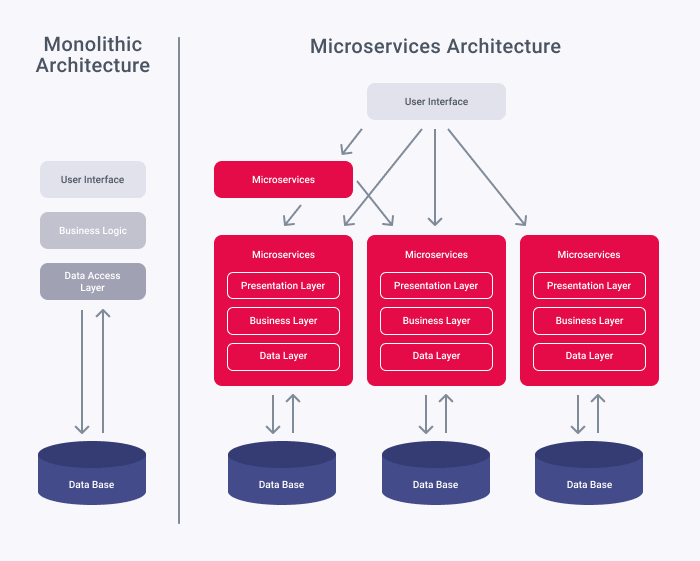
\includegraphics[width=0.85\textwidth]{img/microservice_architecture.png}
			\caption{Comparativa entre arquitectura de microservicios y arquitectura ``monolítica''. [\ref{bib_img: microservice architecture}]}
			\label{img: microservice architecture}
		\end{center}
	\end{figure}
	
	
	\pagebreak
	
	\section{Bases de datos}
	
	\noindent Para asegurar la persistencia de los datos en nuestra aplicación, es necesario utilizar una base de datos. En dicha base de datos, guardaremos información relevante para el correcto funcionamiento del sistema, en nuestro caso, redes y/o interfaces a monitorizar, o los datos monitorizados. \\
	
	\noindent En la aplicación de monitorización, distinguimos entre datos de dos tipos:
	
	\begin{itemize}
		\item Datos clásicos. Como por ejemplo, la información asociada a una red a monitorizar.
		\item Datos de tipo ''serie temporal''. Como por ejemplo, las muestras de monitorización de una red.
	\end{itemize}

	\noindent En primer lugar, se diseña una base de datos tipo relacional para almacenar los ''datos clásicos''. Y por otro lado, se diseña una base de datos diferente, especializada para el almacenamiento de datos tipo ''serie de datos'', en este caso, se elige una base de datos llamada InfluxDB.
	
	\subsection{Base de datos tipo relacional}
	
	\noindent Un ejemplo de base de datos de tipo relacional es SQL. Dicha base de datos, supone una colección de información que organizan los datos en una serie de ''relaciones'' cuando la información es almacenada en una o varias ''tablas''. Por lo tanto, las relaciones suponen conexiones entre diferentes tablas, permitiendo así una asociación entre información diferente. [\ref{bib: relational database}] \\
	
	\noindent Por ejemplo, si vemos la figura \ref{img: example sql}, podemos comprobar como se realizan las relaciones entre las diferentes tablas (Ratings, Users, Movies o Tags), se realiza mediante uno de los campos definidos en la propia tabla. Por ejemplo, el campo ''user\_id'' de la tabla Ratings, permite una relación con la tabla Users, con el campo ''id''.
	
	\begin{figure}[h!]
		\begin{center}
			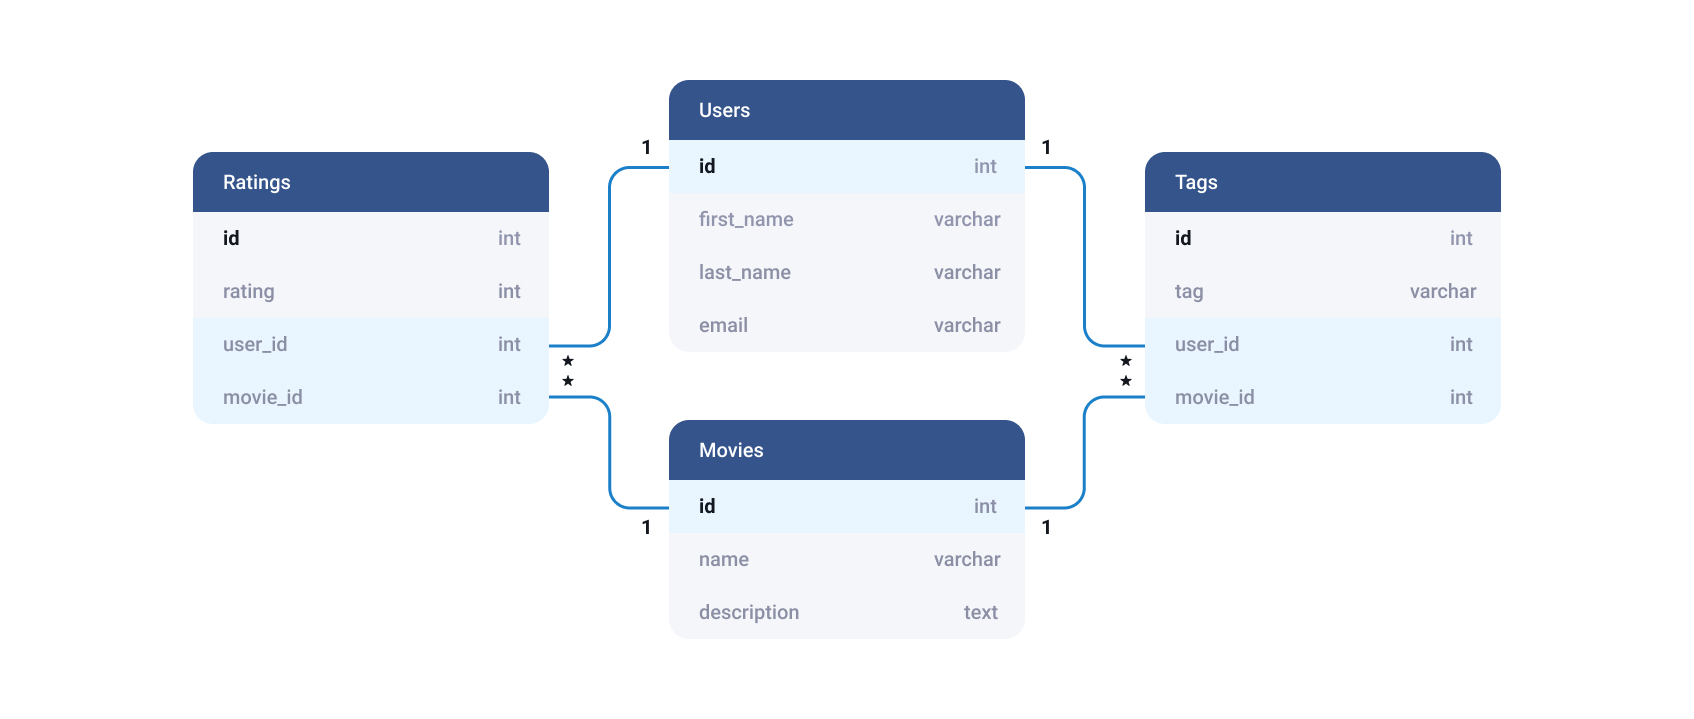
\includegraphics[width=0.95\textwidth]{img/example_relational_database.jpg}
			\caption{Ejemplo de relaciones dentro de una base de datos SQL. [\ref{bib_img: example sql}]}
			\label{img: example sql}
		\end{center}
	\end{figure}
	
	\noindent Para el caso de nuestra aplicación de monitorización de tráfico en red, modelamos la base de datos según la información que vamos a almacenar. Por lo que tenemos que definir la estructura de tablas, los campos que van a tener cada una de las tablas, y los campos por los que se van a relacionar entre sí. A esta información la llamamos modelo de datos.
	
	
	
	\pagebreak
	
	\subsection{Base de datos tipo ``serie temporal''} 
	
	\noindent InfluxDB es una base de datos diseñada para trabajar con datos tipo serie temporal (\texttt{time series}). Si bien es cierto que SQL puede gestionar este tipo de datos, no fue creado estrictamente para este objetivo. En este caso, InfluxDB esta diseñado para almacenar grandes volúmenes de datos, y además realizar análisis en tiempo real sobre esos datos. \\
	
	\noindent En comparación con SQL, en InfluxDB un ``timestamp'' identifica un punto en cualquier serie de datos. Esto sería equivalente a SQL, si la clave primaria de una tabla es establecida por el sistema y siempre es equivalente al tiempo. Además, InfluxDB permite reconocer el ``schema'' de manera dinámica, además de que no estas obligado a definir el ``schema'' y seguirlo, es decir, se permiten cambios dentro de la misma serie de datos. [\ref{bib: influxdb doc vs sql}] \\
	
	\noindent Algunas de las razones destacadas para elegir InfluxDB son: [\ref{bib: influxdb doc}]
	
	\begin{itemize}
		\item Perfecto para almacenar datos de telemetría, como métricas de aplicaciones o sensores IoT.
		\item Los datos son comprimidos automáticamente para ser eficientes con el espacio disponible.
		\item Se realizan tareas automáticas de ``down sampling'' para reducir el uso de disco.
		\item Lenguaje para hacer consultas que permite analizar en profundidad los datos almacenados.
		\item Disponible una aplicación web para realizar consultas y comprobar los datos disponibles en la base de datos.
	\end{itemize}

	\vspace{10px}

	\noindent \textbf{\large Terminología} \\
	
	\noindent Comparando con los conceptos ya existentes en bases de datos de tipo SQL, se definen los siguientes conceptos en InfluxDB:
	
	\begin{itemize}
		\item ``measurement'': equivalente a una tabla.
		\item ``tags'': equivalente a columnas indexadas dentro de una tabla.
		\item ``fields'': equivalente a columnas no indexadas dentro de una tabla.
		\item ``points'': similar a las filas en una tabla.
	\end{itemize}

	\vspace{20px}

	\begin{figure}[h!]
		\begin{center}
			
\includegraphics[width=0.6\textwidth]{img/InfluxDB.png}
			\caption{Logotipo base de datos InfluxDB [\ref{bib_img: influxdb logo}].}
			\label{img: influxdb logo}
		\end{center}
	\end{figure}
	
	\pagebreak
	
	\section[Lenguajes y frameworks]{Lenguajes de programación y frameworks}
	
	\noindent En resumen, para el desarrollo de esta aplicación se ha utilizado el lenguaje de programación Python, con el framework de desarrollo para APIs llamado FastAPI.
	
	\subsection{Python}
	
	\noindent Python [\ref{bib: python doc}] es un lenguaje de programación orientado a objetos, interpretado y de alto nivel con tipado dinámico. Es muy atractivo ya que permite un desarrollo rápido de aplicaciones, además de ser muy adecuado para realizar tareas de ``scripting''. Python es un lenguaje simple y sencillo de aprender. Por otro lado, dispone de multitud de ``librerías'' o ``módulos'' publicados por usuarios, dando lugar a una gran comunidad y una gran variedad de alternativas para implementar soluciones. \\
	
	\noindent Actualmente, Python destaca como lenguaje de programación en los siguientes ámbitos:
	\begin{itemize}
		\item Desarrollo de aplicaciones web, utilizando los frameworks Django, Flask o FastAPI.
		\item Tareas asociadas a ``data science'', utilizando librerías como Pandas o NumPy.
		\item Inteligencia artificial, utilizando frameworks como TensorFlow o scikit-learn.
	\end{itemize}
	
	\begin{figure}[h!]
		\begin{center}
			
\includegraphics[width=0.5\textwidth]{img/python_logo.png}
			\caption{Logotipo Python [\ref{bib_img: python logo}].}
			\label{img: python logo}
		\end{center}
	\end{figure}
	
	\subsection{FastAPI}
	\label{sec: fastapi}
	
	\noindent FastAPI [\ref{bib: fastapi doc}] es un framework moderno y rápido para construir APIs utilizando la versión de Python 3.7+. Algunas de las características más destacadas son:
	
	\begin{itemize}
		\item Rápido: rendimiento muy alto, prácticamente a la par con otros lenguajes de programación destinados al desarrollo de \texttt{backend} (como NodeJS o Go).
		\item Intuitivo: soporta auto completado en el código.
		\item Robusto: código pensado para entornos de producción, además de incluir documentación automática (usando Swagger o ReDoc).
		\item Basado en estándares: al utilizar estándares de tipo de datos, permite ser totalmente compatible con los estándares de \href{https://github.com/OAI/OpenAPI-Specification}{OpenAPI} [\ref{bib: openapi}] y \href{https://json-schema.org/}{JSON Schema} [\ref{bib: json schema}].
	\end{itemize}
	
	\pagebreak
	
	\begin{figure}[h!]
		\begin{center}
			
\includegraphics[width=0.6\textwidth]{img/fastapi_logo.png}
			\caption{Logotipo FastAPI [\ref{bib_img: fastapi logo}].}
			\label{img: fastapi logo}
		\end{center}
	\end{figure}

	\subsection{Prophet}
	\label{sec: prophet}
	
	\noindent Prophet [\ref{bib: prophet doc}] es un framework del lenguaje de programación Python, desarrollado por \href{https://github.com/facebook/}{Meta}, que recoge una serie de procedimientos que permiten realizar predicciones de un \texttt{dataset} de series temporales, en el que se pueden encontrar diferentes efectos no lineales, llamados tendencias (como puede ser una tendencia anual, semanal, o mensual), además de otros efectos causados por fechas concretas. \\
	
	\noindent Es un framework de predicción basado en inferencia estadística, lo que permite tener un rendimiento mayor que si utilizamos técnicas de Machine Learning para solucionar el mismo problema de predicción de datos. Además, es robusto a datos no disponibles y a modificaciones aleatorias sobre las tendencias. 
	
	\begin{figure}[h!]
		\begin{center}
			
\includegraphics[width=0.55\textwidth]{img/prophet_logo.png}
			\caption{Logotipo Prophet [\ref{bib_img: prophet logo}].}
			\label{img: prophet logo}
		\end{center}
	\end{figure}
	
	\pagebreak
	
	\section[Despliegue en producción]{Tecnologías utilizadas en un despliegue en producción}
	
	\noindent Otro de los aspectos importantes para la realización de este proyecto, es el hecho de que la aplicación desarrollada debe ser apta para desplegarse en un entorno de producción y funcionar correctamente para que sea implementada como microservicio por otras aplicaciones. Es por este motivo por el que nos decantamos por implementar este microservicio dentro de un contenedor. \\
	
	\noindent \textbf{\large Docker} \\

	\noindent Utilizamos Docker como la tecnología para realizar un contenedor de nuestra aplicación, implementando dentro del contenedor todas las librerías y código necesario para hacer funcionar la aplicación. \\
	
	\noindent Por otro lado, también será necesario desplegar diferentes contenedores que tendrán alojadas las bases de datos que utilizaremos en el proyecto. En este caso, al utilizar dos bases de datos, tendremos que hacer uso de un contenedor para desplegar una base de datos SQL, y otro contenedor para desplegar una base de datos InfluxDB. \\ 
	
	\noindent Los contenedores Docker necesarios se desplegarán sobre una máquina host que tenga en funcionamiento el ``daemon'' de Docker. Ver figura \ref{img: docker arch}.
	
	\begin{figure}[h!]
		\begin{center}
			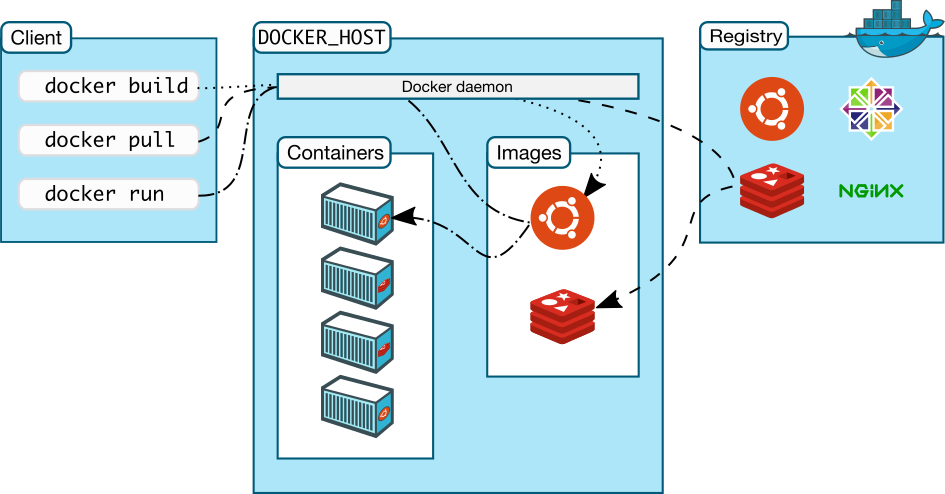
\includegraphics[width=0.95\textwidth]{img/architecture-docker.png}
			\caption{Arquitectura de Docker. [\ref{bib_img: docker architecture}]}
			\label{img: docker arch}
		\end{center}
	\end{figure}

	\pagebreak
	
	\noindent \textbf{\large Docker Compose} \\
	
	\noindent Compose es una herramienta de Docker que permite definir y ejecutar instancias multicontenedores de Docker [\ref{bib: docker compose doc}]. Con la herramienta Compose, podemos utilizar un archivo YAML para describir y configurar los contenedores que vamos a utilizar, dando lugar a que con un único comando puedas crear y ejecutar todos los servicios de la aplicación, y con la misma configuración. \\
	
	\noindent Compose funciona para los diferentes entornos: producción, desarrollo, y o pruebas. Además, tiene disponibles comandos para hacer más sencilla la tarea de iniciar o parar servicios, o ver la salida de consola producida por los contenedores. \\
	
	\noindent En el caso de nuestra aplicación, el archivo ``\textit{docker-compose.yml}'' utilizado para el entorno de desarrollo sería el siguiente:
	
	\begin{lstlisting}[style=yaml, caption={Archivo configuración de contenedores para entorno de desarrollo.}]
version: '3.8'

services:
  traffic_forecast:
    build: ./backend
    ports:
     - 5000:5000
    environment:
     - POSTGRES_USER=monitor
     - POSTGRES_PASSWORD=forecast2022
     - POSTGRES_DB=traffic-forecast
     - INFLUX_TOKEN=*******
     - INFLUX_ORG=e-lighthouse
     - INFLUX_BUCKET=traffic-forecast
     - SECRET_KEY=upct2022_sk
     - FASTAPI_CONFIG=development
    volumes:
     - ./backend:/app
    depends_on:
     - db
     - influxdb

  db:
    image: postgres:13
    expose:
     - 5432
    environment:
     - POSTGRES_USER=monitor
     - POSTGRES_PASSWORD=forecast2022
     - POSTGRES_DB=traffic-forecast
    volumes:
     - ./data/postgres_db:/var/lib/postgressql/data
    
   influxdb:
     image: influxdb:latest
     volumes:
       - ./data/influxdb/data:/var/lib/influxdb2:rw
     ports:
       - 8086:8086
	\end{lstlisting}

	\pagebreak
	
	\noindent Para desplegar los contenedores, según el archivo YAML definido, tenemos que ejecutar el siguiente comando: 
	
	\begin{verbatim}
		docker compose up -f <filename> traffic_forecast
	\end{verbatim}
	
	\noindent \textbf{\large Traefik} \\
	
	\noindent Traefik es una herramienta que permite hacer de ``reverse proxy'' y ``load balancer'' en contenedores Docker, permitiendo el despliegue sencillo de microservicios en un entorno de producción. \\
	
	\noindent Traefik esta diseñado para ser simple de operar, pero con una gran capacidad de gestión en entornos complejos. Además, se integra perfectamente con la infraestructura ya existente y configurar el sistema de manera dinámica. Algunas de las tareas que realiza Traefik son: [\ref{bib: traefik webpage}] 
	
	\begin{itemize}
		\item Gestionar ``middlewares'' necesarios para la aplicación (forzar protocolos específicos, configurar contraseña para el servicio...).
		\item Funcionar como API ``gateway'', gestionando los dominios y certificados para cada uno de los microservicios desplegados.
		\item Orquestador de nodo de entrada, gestionando la comunicación de tráfico de un dominio hacia el servicio asociado.
	\end{itemize}

	\begin{figure}[h!]
		\begin{center}
			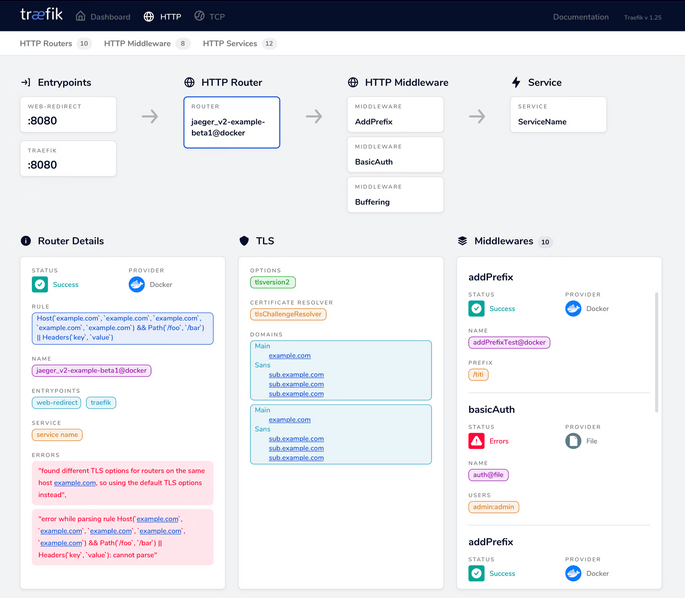
\includegraphics[width=0.78\textwidth]{img/traefik_example.png}
			\caption{Captura portal de gestión de Traefik. Detalle del enrutado hacia un servicio. [\ref{bib_img: traefik capture}]}
		\end{center}
	\end{figure}
	
	\pagebreak
	
	\noindent En el caso de nuestra aplicación, para el entorno de producción usamos el siguiente archivo que permite a la herramienta docker compose ejecutar los servicios con sus configuraciones asociadas. Como podemos ver, en la sección de ``labels'' se encuentra la configuración asociada a Traefik. Dicha configuración permite a Traefik asignar un servicio a un dominio, crear un certificado SSL y configurar los puertos de acceso para dicho servicio. [\ref{bib: traefik wiki}]
	
	\begin{lstlisting}[style=yaml, caption={Archivo configuración de contenedores para entorno de producción.}]
version: '3.8'

services:
  traffic_forecast:
    build: ./backend
    container_name: traffic_forecast-api
    restart: unless-stopped
    environment:
      - POSTGRES_USER=monitor
      - POSTGRES_PASSWORD=forecast2022
      - POSTGRES_DB=traffic-forecast
      - INFLUX_URL=https://tfm-influx.ranii.pro:8443/
      - INFLUX_TOKEN=****
      - INFLUX_ORG=e-lighthouse
      - INFLUX_BUCKET=traffic-forecast
      - SECRET_KEY=upct2022_sk
    volumes:
      - ./backend:/app
    labels:
      - traefik.enable=true
      - traefik.http.routers.tf-api.entryPoints=web-secure
      - traefik.http.routers.tf-api.rule=Host(`tfm-api.ranii.pro`)
      - traefik.http.routers.tf-api.tls.certresolver=default
      - traefik.http.services.tf-api.loadbalancer.server.port=5000
    depends_on:
      - db
      - influxdb

  db:
    image: postgres:13
    container_name: traffic_forecast-postgres
    restart: unless-stopped
    environment:
      - POSTGRES_USER=monitor
      - POSTGRES_PASSWORD=forecast2022
      - POSTGRES_DB=traffic-forecast
    volumes:
      - ./data/postgres_db:/var/lib/postgressql/data

  influxdb:
    image: influxdb:latest
    container_name: traffic_forecast-influx
    restart: unless-stopped
    volumes:
      - ./data/influxdb/data:/var/lib/influxdb2:rw
    labels:
      - traefik.enable=true
      - traefik.http.routers.tf-influx.entryPoints=web-secure
      - traefik.http.routers.tf-influx.rule=Host(`tfm-influx.ranii.pro`)
      - traefik.http.routers.tf-influx.tls.certresolver=default
      - traefik.http.services.tf-influx.loadbalancer.server.port=8086
	\end{lstlisting} 

	\noindent Para desplegar los contenedores, según el archivo YAML definido, tenemos que ejecutar el siguiente comando: 
	
	\begin{verbatim}
		docker compose up -f <filename> traffic_forecast
	\end{verbatim}

	\noindent En el caso de querer profundizar más en el funcionamiento de Traefik, se puede consultar el siguiente enlace \href{https://doc.traefik.io/traefik/}{Traefik: Get Started}
	
	\chapter{Diseño e implementación del sistema}
	
	\noindent En este capítulo se va a comentar más en detalle la implementación del sistema propuesto para la monitorización y predicción de tráfico de red. Tal y como vimos en el capitulo anterior, se va a utilizar el lenguaje de programación Python, con el framework de desarrollo FastAPI.
	
	\section{Descripción API REST}
	
	\noindent Tal y como pudimos ver en la sección \ref{sec: api}, para la aplicación propuesta hemos elegido que siga la estructura de API REST, ya que es la más sencilla de implementar y la más flexible. \\
	
	\noindent Para nuestro caso particular de monitorización del tráfico de una red, se han detectado tres ``agentes'' involucrados dentro del sistema. Dichos agentes son los siguientes:
	
	\begin{itemize}
		\item Redes (desde ahora \texttt{networks}). Corresponde con una red en la que queremos monitorizar el tráfico de ciertas interfaces.
		\item Interfaces de red (desde ahora \texttt{interfaces}). Corresponde con las interfaces de red de las que queremos monitorizar su tráfico.
		\item Muestras de monitorización (desde ahora \texttt{samples}). Corresponden con los diferentes datos de monitorización de tráfico asociados a una interfaz.
	\end{itemize}

	\noindent Definidos los agentes, se procede a diseñar el almacenamiento de la información de cada uno de ellos. Para ello, en primer lugar, nos decantamos por aplicar el concepto de CRUD en los agentes \texttt{networks} y \texttt{interfaces}. \\
	
	\noindent \textbf{\large CRUD: \texttt{networks}} \\
	
	\noindent Tal y como se refiere la definición de CRUD (\textbf{C}reate \textbf{R}ead \textbf{U}pdate \textbf{D}elete), en el caso del agente de \texttt{networks}, queremos definir el funcionamiento que tiene que seguir la aplicación cuando queramos referirnos a una red a monitorizar. Además, asumimos que dentro de una misma red podemos tener diferentes interfaces, que también serán dadas de altas en la aplicación. Por lo tanto, una única red puede tener muchas interfaces de red monitorizadas. \\
	
	\noindent Dado que estamos planteando un servicio HTTP, debemos asignar una ruta (desde ahora \texttt{endpoint}) asociada a la colección de métodos de la CRUD de \texttt{networks}. En este caso, el endpoint de la colección sera: ``\texttt{/networks}''
	
	\pagebreak
	
	\noindent A modo de resumen, recogemos en la siguiente tabla el funcionamiento esperado de la aplicación, en función del método HTTP recibido y el recurso sobre el que se ejecute la petición HTTP.
	
	\begin{table}[h!]
		\centering
		\resizebox{\columnwidth}{!}{%
			\begin{tabular}{lllll}
				\hline
				\multicolumn{1}{|c|}{\textbf{Recurso}}                                                                                           & \multicolumn{1}{c|}{\textbf{\texttt{GET}}}                                                                    & \multicolumn{1}{c|}{\textbf{\texttt{POST}}}                                                  & \multicolumn{1}{c|}{\textbf{\texttt{PATCH}}}                                                                      & \multicolumn{1}{c|}{\textbf{\texttt{DELETE}}}                                               \\ \hline
				\multicolumn{1}{|l|}{\begin{tabular}[c]{@{}l@{}}Colección de redes:\\ \\ \texttt{/networks}\end{tabular}}                                 & \multicolumn{1}{l|}{\begin{tabular}[c]{@{}l@{}}Lista de redes \\ dadas de alta\end{tabular}}         & \multicolumn{1}{l|}{\begin{tabular}[c]{@{}l@{}}Añade una nueva \\ red\end{tabular}} & \multicolumn{1}{c|}{*}                                                                                   & \multicolumn{1}{c|}{*}                                                             \\ \hline
				\multicolumn{1}{|l|}{\begin{tabular}[c]{@{}l@{}}Red en particular:\\ \\ \texttt{/networks/\textless{}id\_net\textgreater{}}\end{tabular}} & \multicolumn{1}{l|}{\begin{tabular}[c]{@{}l@{}}Información de\\  una red en particular\end{tabular}} & \multicolumn{1}{c|}{*}                                                              & \multicolumn{1}{l|}{\begin{tabular}[c]{@{}l@{}}Modificamos la \\ informacion de \\ una red\end{tabular}} & \multicolumn{1}{l|}{\begin{tabular}[c]{@{}l@{}}Eliminamos \\ una red\end{tabular}} \\ \hline
				&                                                                                                      &                                                                                     &                                                                                                          &                                                                                   
			\end{tabular}%
		}
		\caption{CRUD \texttt{networks} (* equivale a ``acceso denegado'')}
		\label{tab:crud networks}
	\end{table}

	\vspace{22px}

	\noindent \textbf{\large CRUD: \texttt{interfaces}} \\
	
	\noindent Para el caso del agente \texttt{interfaces}, definimos el funcionamiento de la aplicación. Entendemos una interfaz como aquellas interfaces de red que queremos monitorizar su tráfico dentro de una red, que previamente ya ha sido dada de alta en el sistema. \\
	
	\noindent Cómo compromiso de diseño, se entiende que de cada interfaz tendremos que dar de alta dos interfaces en el sistema, una interfaz para monitorizar los datos de transmisión (desde ahora, TX) y otra interfaz para monitorizar los datos de recepción (desde ahora, RX). De esta manera, tendríamos completamente monitorizada la interfaz de red. \\
	
	\noindent Una interfaz monitorizada puede tener muchas muestras guardadas en el sistema, dichas muestras serán almacenadas en la base de datos para datos temporales (en nuestro caso InfluxDB). \\
	
	\noindent Al igual que en el caso de \texttt{networks}, debemos asignar un \texttt{endpoint} asociado a la colección de los métodos CRUD de \texttt{interfaces}. En este caso, el \texttt{endpoint} asociado de la colección será: ``\texttt{/networks/<id\_net>/interfaces}''. \\
	
	\begin{table}[h!]
		\centering
		\resizebox{\columnwidth}{!}{%
			\begin{tabular}{|l|l|c|c|c|}
				\hline
				\multicolumn{1}{|c|}{\textbf{Recurso}}                                                                                                                     & \multicolumn{1}{c|}{\textbf{\texttt{GET}}}                                                        & \textbf{\texttt{POST}}                                                                                      & \textbf{\texttt{PATCH}}                                                                                                 & \textbf{\texttt{DELETE}}                                                                         \\ \hline
				\begin{tabular}[c]{@{}l@{}}Colección de interfaces:\\ \\ \texttt{/networks/\textless{}id\_net\textgreater{}/interfaces}\end{tabular}                                & \begin{tabular}[c]{@{}l@{}}Listado de \\ interfaces dentro \\ de una red.\end{tabular}   & \multicolumn{1}{l|}{\begin{tabular}[c]{@{}l@{}}Añade una nueva\\ interfaz a una red.\end{tabular}} & *                                                                                                              & *                                                                                       \\ \hline
				\begin{tabular}[c]{@{}l@{}}Interfaz en particular:\\ \\ \texttt{/networks/\textless{}id\_net\textgreater{}/interfaces/\textless{}id\_if\textgreater{}}\end{tabular} & \begin{tabular}[c]{@{}l@{}}Información \\ de una interfaz \\ en particular.\end{tabular} & *                                                                                                  & \multicolumn{1}{l|}{\begin{tabular}[c]{@{}l@{}}Modificamos \\ la información \\ de una interfaz.\end{tabular}} & \multicolumn{1}{l|}{\begin{tabular}[c]{@{}l@{}}Eliminamos \\ una interfaz\end{tabular}} \\ \hline
			\end{tabular}%
		}
		\caption{CRUD \texttt{interfaces} (* equivale a ``acceso denegado'')}
		\label{tab:crud interfaces}
	\end{table}

	\pagebreak

	\noindent \textbf{\large Métodos no CRUD} \\
	
	\noindent Por otro lado, la aplicación también estará compuesta por otros métodos que no encajan en el esquema CRUD. Estos métodos son:
	
	\begin{itemize}
		\item Muestras monitorizadas. Permite importar muestras al sistema. Corresponde con el \texttt{endpoint}: \texttt{/samples}
		\item Consultas de muestras monitorizadas. Permite acceder a la información de monitorización que esta almacenada en el sistema. Corresponde con el \texttt{endpoint}: \texttt{/query}
		\item Ejecución de una predicción. Permite generar una predicción de tráfico. Corresponde con el \texttt{endpoint}: \texttt{/forecast}
	\end{itemize}
	
	\vspace{22px}
	
	\noindent \textbf{\large Resumen arquitectura de la aplicación} \\
	
	\noindent En la figura \ref{img: app schema} podemos ver un resumen de la estructura de la aplicación propuesta. En verde aparecen las rutas que siguen una estructura CRUD, en azul las rutas que no tienen por qué seguir la estructura CRUD, y a la derecha podemos ver las dos bases de datos necesarias (una relacional y otra para series temporales de datos).
	
	\begin{figure}[h!]
		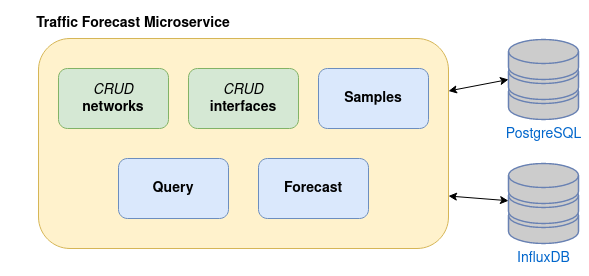
\includegraphics[width=1.1\textwidth, center]{diag/traffic_forecast_schema.png}
		\caption{Diagrama resumen de la estructura de la aplicación.}
		\label{img: app schema}
	\end{figure}

	\pagebreak
	
	\section{Implementación de la aplicación}
	
	\noindent Tal y como se adelantó en la sección \ref{sec: fastapi}, el lenguaje utilizado para implementar la aplicación es Python, utilizando el \texttt{framework} de desarrollo FastAPI. \\
	
	\noindent Para la implementación de la aplicación, se ha seguido la metodología de diseño ``\textit{Factory Pattern}''. Dicha metodología permite estructurar un proyecto software de modo que la implementación de nuevas funcionalidades sea sencilla y no implique modificar partes ya validadas del sistema. Esto se basa en que permitimos a una clase crear objetos derivados de esta, en función de las necesidades del sistema. A grandes rasgos, intentamos emular el funcionamiento de una producción en cadena de una fabrica. Podemos encontrar más información en: [\ref{bib: factory method}] [\ref{bib: fastapi doc bigger apps}]. \\
	
	\noindent A consecuencia de esta metodología, el proyecto se estructura según la imagen \ref{img: folder structure}. Dicha estructura tiene como raíz la carpeta \texttt{backend}, y esta se divide tal que:
	
	\begin{itemize}
		\item \texttt{migrations}. Carpeta que contiene las utilidades asociadas a la migración de la base de datos SQL. Permite realizar modificaciones en los modelos de datos y que dichas modificaciones se apliquen en la base de datos final.
		\item \texttt{src}. Carpeta en la que encontramos todo el código asociado a la aplicación.
			\begin{itemize}
				\item \texttt{crud}. Contiene los archivos de funcionalidad para cada una de las CRUD (\texttt{networks} y \texttt{interfaces}).
				\item \texttt{database}. Contiene los archivos asociados a los modelos de datos.
				\item \texttt{noncrud}. Contiene la funcionalidad de los agentes que no siguen la estructura CRUD (\texttt{samples}, \texttt{query} y \texttt{forecast}).
				\item \texttt{routes}. Contiene los \texttt{endpoints} de la aplicación, redirige a la funcionalidad en las carpetas \texttt{crud} y/o \texttt{noncrud}.
				\item \texttt{schemas}. Contiene los diferentes esquemas de datos que se utilizan en la aplicación, tanto de entrada de datos del usuario, como de salida de datos del sistema.
				\item \texttt{utils}. Contiene funciones de ayuda para simplificar el código, por ejemplo para manejar el InfluxDB.
				\item \texttt{config.py}. Contiene las opciones configurables de la aplicación. Se definen dos entornos de ejecución: \texttt{development} o \texttt{production}.
				\item \texttt{main.py}. Archivo principal del sistema, aquí comienza la ejecución de la aplicación.
			\end{itemize}
		
		\item \texttt{Dockerfile}. Archivo que describe los pasos para crear un contenedor para nuestra aplicación.
		\item \texttt{requirements.txt}. Archivo que contiene los diferentes paquetes de Python utilizados.
	\end{itemize}
	
	\pagebreak
	
	\begin{figure}[h!]
		\begin{center}
			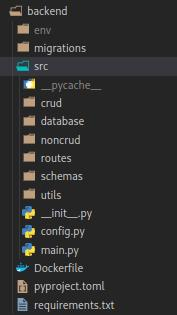
\includegraphics[width=0.3\textwidth]{img/folder_structure.jpg}
			\caption{Captura estructura de carpetas de la aplicación.}
			\label{img: folder structure}
		\end{center}
	\end{figure}

	\noindent De esta manera, en el caso de querer añadir una funcionalidad nueva, solo tendríamos que modificar los archivos pertinentes. Las modificaciones en archivos ya existentes serían mínimas. Permitiendo de esta manera un fácil mantenimiento y desarrollo sobre la aplicación. \\
	
	\subsection{Migración de base de datos tipo relacional}
	
	\noindent Para permitir que sea sencillo extender los modelos de datos de la aplicación es necesario tener en cuenta qué va a suceder si en algún momento decidimos cambiar algo de dichos modelos y qué tenemos que hacer para que esos cambios se apliquen correctamente en la base de datos que estemos utilizando. Es por esto por lo que aparecen dos herramientas muy importantes: \texttt{ORM} y \texttt{migrations}.  \\
	
	\noindent En primer lugar, \texttt{ORM} (Object-relational Mappers) permite una abstracción de alto nivel que da lugar a describir un modelo de datos de SQL en Python, en vez de utilizar lenguaje SQL directamente. Además, permite acceder a la información de la base de datos de manera más sencilla, ya que para el programa es como si el modelo de datos fuera un objeto, pero internamente se están realizando las consultas SQL que sean necesarias. [\ref{bib: orm python}] [\ref{bib: fastapi orm}] \\
	
	\noindent En segundo lugar, \texttt{migrations} permite tener un control de versiones dentro de los modelos de datos que estemos usando en la aplicación. Además, permite aplicar automáticamente modificaciones en los modelos de datos, de modo que al ejecutar la aplicación, la base de datos actualizará su estructura (por ejemplo, añadir una nueva columna en una tabla) en función del modelo de datos que hayamos actualizado del \texttt{ORM}. [\ref{bib: fastapi migrations}]
	
	\pagebreak
	
	\subsection{OpenAPI Specification. \texttt{Swagger}}
	
	\noindent Una de las ventajas que supone el uso de FastAPI, es que de manera automática genera la documentación asociada a OpenAPI de la aplicación, dando lugar a que el endpoint \texttt{/docs} nos redirige directamente a la aplicación web \texttt{Swagger}, que nos muestra de una manera sencilla todos los \texttt{endpoints} asociados de nuestra aplicación, permitiendo realizar peticiones y comprobando la funcionalidad de estas. \\
	
	\noindent De esta manera, si navegamos a dicha ruta (\texttt{/docs}), podemos ver como nos aparece una web similar a la de la figura \ref{img: swagger 1}.
	
	\begin{figure}[h!]
		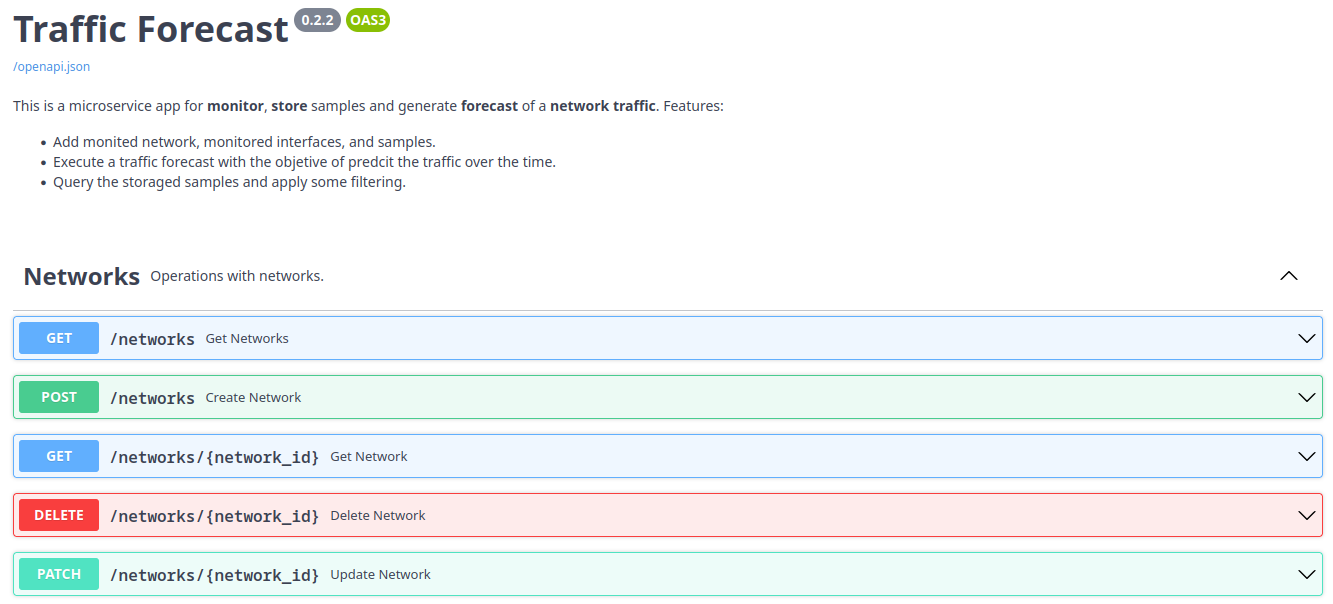
\includegraphics[width=1.2\textwidth,center]{img/swagger_1.png}
		\caption{Captura Swagger. Vista por defecto.}
		\label{img: swagger 1}
	\end{figure}

	\noindent A modo de ejemplo, si hiciéramos \textit{click} en uno de los \texttt{endpoints}, podremos comprobar como se nos despliega información asociada. Por ejemplo, del esquema de datos de entrada, o el esquema de datos de salida, al igual que los códigos HTTP esperados. En la figura \ref{img: swagger 2}, podemos ver el detalle de la información necesaria para crear una red. \\
	
	\noindent Además, una de las funcionalidades más interesantes que nos aporta Swagger, es la documentación necesaria sobre los esquemas de los JSON de salida de la aplicación. Esto es muy importante ya que nos permitiría conectar con otras aplicaciones, y presentar la información recibida. En la figura \ref{img: swagger schemas 1}, podemos ver un detalle de algunos de los esquemas que se utilizan en la aplicación.
	
	\pagebreak
	
	\begin{figure}[h!]
		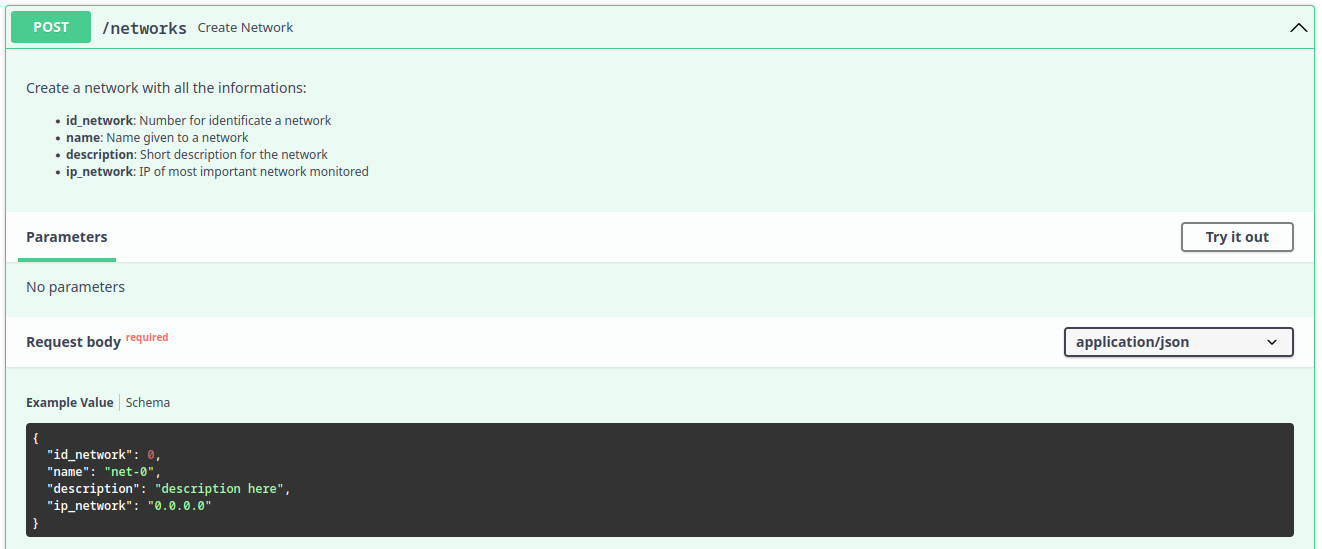
\includegraphics[width=1.2\textwidth, center]{img/swagger_2.png}
		\caption{Captura Swagger. Detalle del método de crear red. (\texttt{POST} a \texttt{/networks})}
		\label{img: swagger 2}
	\end{figure}

	\begin{figure}[h!]
		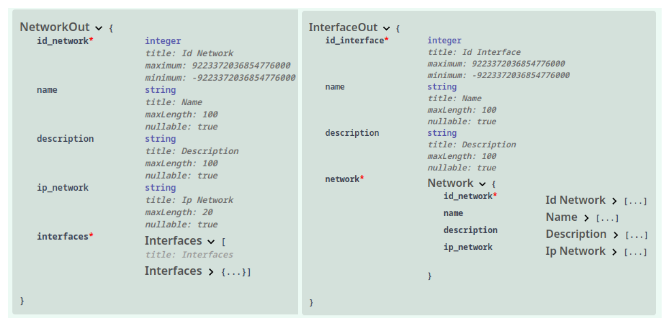
\includegraphics[width=1.2\textwidth, center]{img/swagger_schemas_1.png}
		\caption{Captura Swagger. Detalle esquemas JSON de salida de \texttt{networks} e \texttt{interfaces}.}
		\label{img: swagger schemas 1}
	\end{figure}
	
	
	\pagebreak
	
	\section{Modelos de datos}
	
	\noindent Por otro lado, debemos definir los datos y su representación dentro de nuestra aplicación. Esto nos permite adaptar la información en función del tipo de base de datos que vayamos a consultar, y en función del modelo a utilizar. Para ello, diferenciamos entre los modelos que estarán almacenados en la base de datos de tipo relacional, y los datos almacenados en la base de datos de tipo serie temporal.
	
	\subsection{Base de datos SQL}
	
	\noindent El primer modelo de datos de la aplicación, es el referido a la información de una red a monitorizar. La descripción del modelo la podemos ver en la tabla \ref{tab: modelo sql networks}.
	
	%\begin{figure}[h!]
	%	\begin{center}
	%		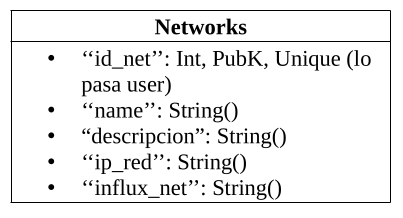
\includegraphics[width=0.45\textwidth]{img/model_sql_networks.png}
	%		\caption{Modelo de datos para las redes a monitorizar. Equivale con la tabla ''networks''.}
	%		\label{img: modelo sql networks}
	%	\end{center}
	%\end{figure}
	
	\begin{table}[h!]
		\centering
		\begin{tabular}{|l|}
			\hline
			\multicolumn{1}{|c|}{\textit{\textbf{Networks}}} \\ \hline
			\texttt{id\_network}: Int, Public Key, Unique                 \\ \hline
			\texttt{name}: String                                     \\ \hline
			\texttt{description}: String                              \\ \hline
			\texttt{ip\_red}: String                                  \\ \hline
			\texttt{influx\_net}: String                              \\ \hline
		\end{tabular}
		\caption{Modelo de datos para las redes a monitorizar. Equivale con la tabla ``networks''.}
		\label{tab: modelo sql networks}
	\end{table}
	
	\vspace{12px}
	
	\noindent El segundo modelo de datos de la aplicación, es el referido a la información de una interfaz a monitorizar, que esta dentro de una red monitorizada. La descripción del modelo la podemos ver en la tabla \ref{tab: modelo sql interfaces}.
	
	%\begin{figure}[h!]
	%	\begin{center}
	%		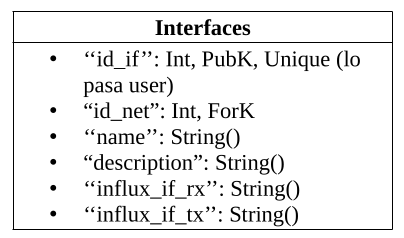
\includegraphics[width=0.45\textwidth]{img/model_sql_interfaces.png}
	%		\caption{Modelo de datos para las interfaces a monitorizar. Equivale con la tabla ''interfaces''}
	%		\label{img: modelo sql interfaces}
	%	\end{center}
	%\end{figure}
	
	\begin{table}[h!]
		\centering
		\begin{tabular}{|l|}
			\hline
			\multicolumn{1}{|c|}{\textit{\textbf{Interfaces}}} \\ \hline
			\texttt{id\_interface}: Int, Public Key, Unique             \\ \hline
			\texttt{name}: String                                       \\ \hline
			\texttt{description}: String                                \\ \hline
			\texttt{influx\_if\_rx}: String                             \\ \hline
			\texttt{influx\_if\_tx}: String                             \\ \hline
			\texttt{network}: Int, Foreign Key                          \\ \hline
		\end{tabular}
		\caption{Modelo de datos para las interfaces a monitorizar. Equivale con la tabla ``interfaces''.}
		\label{tab: modelo sql interfaces}
	\end{table}
	
	\vspace{12px}
	
	\noindent Se establece una relación del modo que una interfaz solo puede pertenecer a una red monitorizada, y que además, una red monitorizada puede tener muchas interfaces. Dicha relación se realiza mediante el campo ``id\_network'' de la tabla Interfaces. \\
	
	\noindent Por último, la base de datos SQL utilizada para esta aplicación es PostgreSQL [\ref{bib: postgresql}], ya que además de ser Open Source, permite una gran escalabilidad, amoldándose a los recursos de la máquina en la que esté funcionando.
	
	\pagebreak
	
	\subsection{Base de datos InfluxDB}
	
	\noindent Para la aplicación a diseñar, se plantea la premisa de que en la base de datos InfluxDB solo se van a guardar los datos de cada muestra de monitorización de una interfaz. Además, se pueden tener tantas redes como sean necesarias, y dentro de cada red, tantas interfaces como creamos necesarias. \\
	
	\noindent En resumen, definimos el modelo de datos que tiene que seguir nuestra aplicación:
	
	\begin{itemize}
		\item ``measurement'': equivalente a una red a monitorizar, valor almacenado en \\ \texttt{Networks::influx\_net}.
		\item ``fields'': nombre del valor a monitorizado, en este caso el default es \textit{link\_count}.
		\item ``tags'': solo tenemos un tag llamado \textit{interface}, su objetivo es identificar a que interfaz pertenece el punto de monitorización. El valor puede estar ser \texttt{Interfaces::influx\_if\_rx} o \texttt{Interfaces::influx\_if\_tx}.
		\item ``points'': corresponde con el valor numérico del ``field''. En este caso, corresponde con el valor númerico de \textit{link\_count} en ese periodo de 5 minutos.
	\end{itemize}

	\section{Predicción de tráfico de red}
	\label{sec: prophet info}
	
	\noindent Uno de los objetivos más importantes que tiene satisfacer la aplicación es la posibilidad de predecir tráfico de red a partir de muestras de monitorización almacenadas en el sistema. Para ello, tal y como introducimos en \ref{sec: prophet}, vamos a utilizar la herramienta de predicción Prophet. \\
	
	\noindent En primer lugar, se decide que la predicción de tráfico va a consumir información que está almacenada en el sistema. Por lo tanto, es necesario crear una red a la que monitorizar, y añadir muestras asociadas a la monitorización. En resumen, si quisiéramos ejecutar una predicción de tráfico desde cero, tendríamos que seguir los siguientes pasos dentro de la aplicación:
	
	\begin{enumerate}
		\item Creamos una red a monitorizar. Utilizaremos el endpoint POST: \texttt{/networks}.
		
		\item Creamos una interfaz a monitorizar, dentro de la red previa. Utilizamos el endpoint POST: \texttt{/networks/<network\_id>/interfaces}.
		
		\item Importamos datos de monitorización. Utilizamos alguno de los endpoints asociados para importar datos, por ejemplo: 
		\begin{itemize}
			\item \texttt{/samples/<network\_id>/import\_topology}
			
			\item \texttt{/samples/<network\_id>/import\_interface/<interface\_id>}
		\end{itemize}
	
		\item Ejecutamos una predicción de tráfico. Usamos el endpoint POST: \texttt{/forecast}. El sistema recuperará las muestras de la interfaz solicitada, y además aplicará un percentil 95, permitiendo así un mejor \texttt{long term estimation}.
	\end{enumerate}

	\noindent Llegados a este punto, una vez ejecutada la predicción y en el caso de que la predicción pueda completarse, el sistema nos devolverá los puntos asociados con toda la serie temporal, incluidos los valores predichos por el sistema. Como característica adicional, se ha implementado la posibilidad de elegir si queremos la salida de los datos como CSV o como JSON.

	\pagebreak

	\noindent En el último paso, en el que ejecutamos la predicción de tráfico, podemos configurar en cierta manera cómo se va a realizar la predicción. Los parámetros a configurar son los siguientes: (ver figura \ref{img: prophet schema})
	
	\begin{itemize}
		\item \texttt{id\_network}. Identificador de red, se obtiene una vez creas la red a monitorizar o haciendo un GET a \texttt{/networks}.
		
		\item \texttt{id\_interface}. Identificador de interfaz de red, es necesario que este asociado con una red a monitorizar. Se obtiene una vez se crea la interfaz, o bien haciendo un GET a \texttt{/networks/<id\_network>/interfaces}.
		
		\item \texttt{field}. Permite seleccionar el tráfico de una interfaz, elegimos entre recepción (``\texttt{RX}'') o transmisión (``\texttt{TX}'').
		
		\item \texttt{days}. Número de días que queremos predecir. Si quisiéramos predecir el tráfico dentro de un año, pondremos \texttt{365}.
		
		\item \texttt{options}. Opciones configurables del modelo de predicción de tráfico. [\ref{bib: prophet parameters}]
		
		\begin{itemize}
			\item \texttt{holidays\_region}. Permite elegir que días festivos se aplican en la predicción. Esto permite detectar sucesos en días de festividad de las diferentes regiones. En el caso de España, tendremos que utilizar ``\texttt{ES}''.
			
			\item \texttt{flexibility\_trend}. Parámetro que más impacto tiene en la predicción. Determina la flexibilidad respecto a una tendencia, es decir, cuanto puede cambiar una tendencia en los diferentes puntos. El valor por defecto es \texttt{0.05}, aunque se puede modificar en un rango de \texttt{[0.001, 0.5]}. Es un parámetro que afecta a la penalización por regulación. [\ref{bib: prophet trend flex}]
			
			\item \texttt{flexibility\_season}. Controla la flexibilidad de los efectos estacionales. El valor por defecto es \texttt{10}, aunque se puede modificar en un rango de \texttt{[0.01, 10]}.
			
			\item \texttt{flexibility\_holidays}. Controla la flexibilidad de los efectos por días festivos. El valor por defecto es \texttt{10}, aunque se puede modificar en un rango de \texttt{[0.01, 10]}.
		\end{itemize}
	\end{itemize}
	
	\begin{figure}[h!]
		\begin{center}
			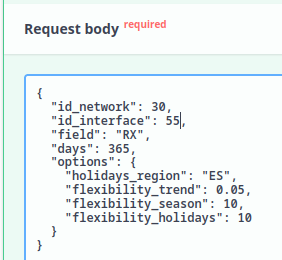
\includegraphics[width=0.4\textwidth]{img/prophet_schema.png}
			\caption{Datos de entrada para la ejecución de una predicción de tráfico.}
			\label{img: prophet schema}
		\end{center}
	\end{figure}

	\pagebreak
	
	\section{Rutas HTTP (\texttt{endpoints})}
	
	\noindent En esta sección se pretende recapitular todos los \texttt{endpoints} disponibles en la aplicación, además de sus esquemas de entrada y de salida. Es importante recordar que la aplicación tiene la herramienta documental \texttt{Swagger} implementada, por lo que accediendo a la ruta \texttt{/doc}, podemos ver toda la documentación asociada a la API.
	
	\subsection{Colección \texttt{Networks}}
	
	\begin{enumerate}
		\item Ruta \texttt{/networks}:
		
		\begin{itemize}
			\item \textbf{Método HTTP}: \texttt{GET}
			\item \textbf{Descripción}: permite listar todas las redes monitorizadas del sistema.
			
			\begin{figure}[h!]
				\begin{center}
					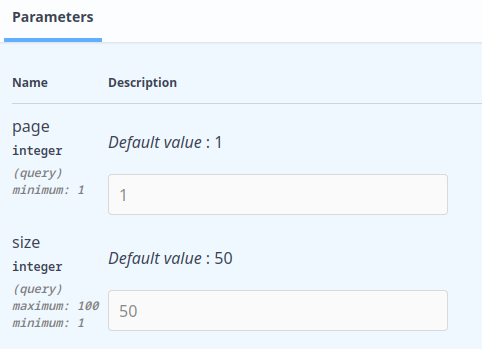
\includegraphics[width=0.38\textwidth]{img/parameters_get_networks.png}
					\caption{Parametros GET Networks}
					\label{img: parameters get networks}
				\end{center}
			\end{figure}
			
			\begin{figure}[h!]
				\begin{center}
					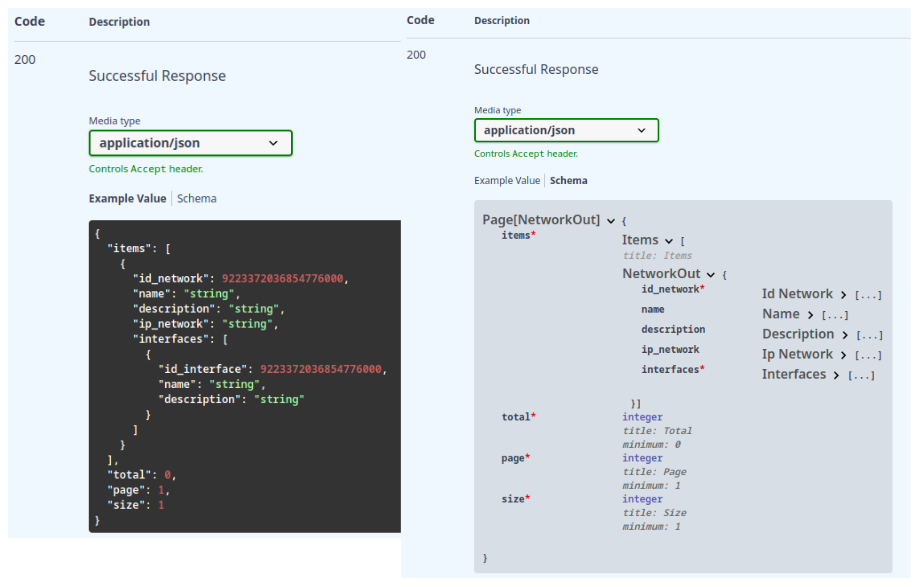
\includegraphics[width=0.87\textwidth]{diag/response_get_networks.png}
					\caption{Respuesta GET Networks}
					\label{img: response get networks}
				\end{center}
			\end{figure}
		
		\end{itemize}
	
		\pagebreak
	
		\item Ruta \texttt{/networks}:
		
		\begin{itemize}
			\item \textbf{Método HTTP}: \texttt{POST}
			\item \textbf{Descripción}: permite crear una nueva red en el sistema.
			
			\begin{figure}[h!]
				\begin{center}
					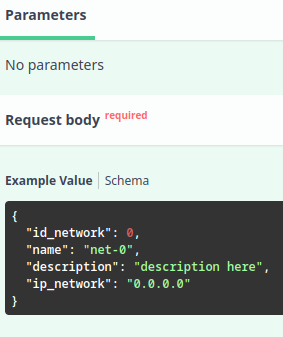
\includegraphics[width=0.35\textwidth]{img/parameters_post_networks.png}
					\caption{Parametros POST Networks}
					\label{img: parameters post networks}
				\end{center}
			\end{figure}
			
			\begin{figure}[h!]
				\begin{center}
					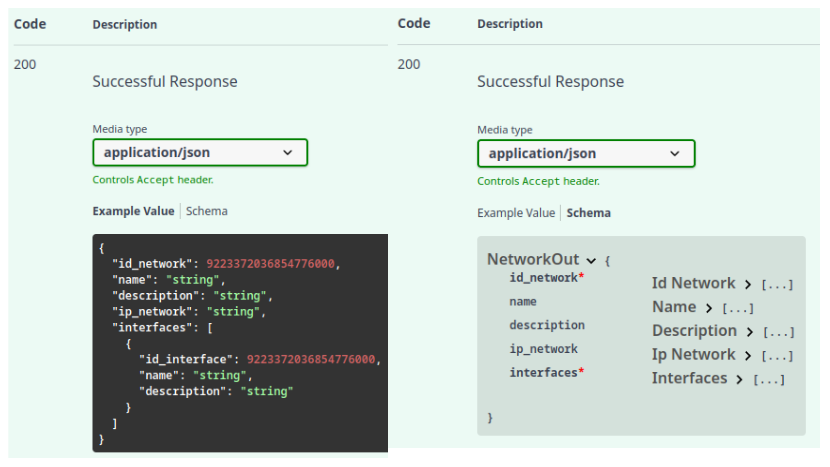
\includegraphics[width=1\textwidth]{diag/response_post_networks.png}
					\caption{Respuesta POST Networks}
					\label{img: response post networks}
				\end{center}
			\end{figure}
		\end{itemize}
	
		\pagebreak
		
		\item Ruta \texttt{/networks/\{network\_id\}}:
		
		\begin{itemize}
			\item \textbf{Método HTTP}: \texttt{GET}
			\item \textbf{Descripción}: devuelve la información de una red, dado un identificador de red.
			\item \textbf{Parámetros}: \texttt{network\_id}, como identificador de red.
			
			\begin{figure}[h!]
				\begin{center}
					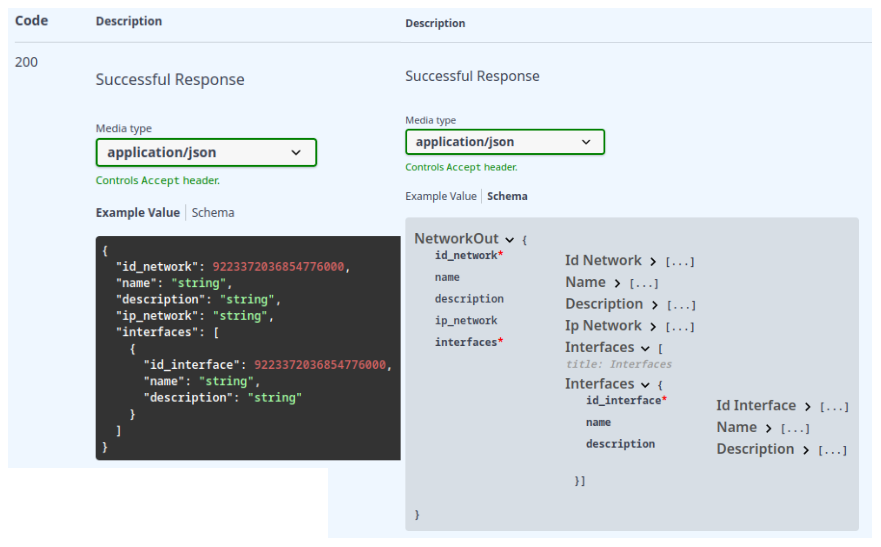
\includegraphics[width=0.85\textwidth]{diag/response_get_network.png}
					\caption{Respuesta GET Network}
					\label{img: response get network}
				\end{center}
			\end{figure}
		\end{itemize}
	
		\item Ruta \texttt{/networks/\{network\_id\}}:
		
		\begin{itemize}
			\item \textbf{Método HTTP}: \texttt{DELETE}
			\item \textbf{Descripción}: elimina una red del sistema, dado un identificador de red. 
			\item \textbf{Parámetros}: \texttt{network\_id}, como identificador de red.
			
			\begin{figure}[h!]
				\begin{center}
					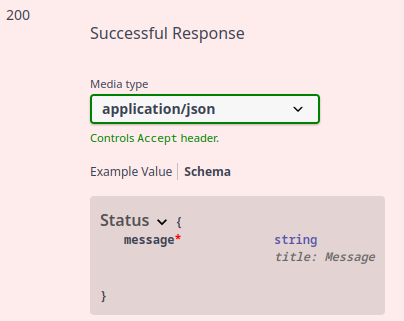
\includegraphics[width=0.4\textwidth]{img/response_delete_network.png}
					\caption{Respuesta DELETE Network}
					\label{img: response delete network}
				\end{center}
			\end{figure}
		\end{itemize}
	
		\pagebreak
		
		\item Ruta \texttt{/networks/\{network\_id\}}:
		
		\begin{itemize}
			\item \textbf{Método HTTP}: \texttt{PATCH}
			\item \textbf{Descripción}: actualiza una red del sistema, dado un identificador de red. 
			\item \textbf{Parámetros}: \texttt{network\_id}, como identificador de red.
			\item \textbf{Respuesta}: equivalente a \ref{img: response get network}, con la información ya modificada.
			
			\begin{figure}[h!]
				\begin{center}
					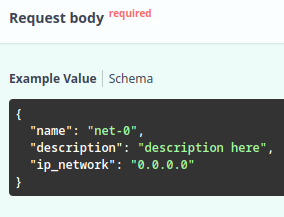
\includegraphics[width=0.35\textwidth]{img/parameters_patch_networks.png}
					\caption{Parámetros PATCH Network}
					\label{img: parameters patch network}
				\end{center}
			\end{figure}
		\end{itemize}
	
	\end{enumerate}
	
	\subsection{Colección \texttt{Interfaces}}
	
	\begin{enumerate}
		\item Ruta \texttt{/networks/\{network\_id\}/interfaces}:
	
		\begin{itemize}
			\item \textbf{Método HTTP}: \texttt{GET}
			\item \textbf{Descripción}: devuelve un listado de interfaces asociadas a una red.
			\item \textbf{Parámetros}: \texttt{network\_id}, como identificador de red. Similar a figura \ref{img: parameters get networks}.
			
			\begin{figure}[h!]
				\begin{center}
					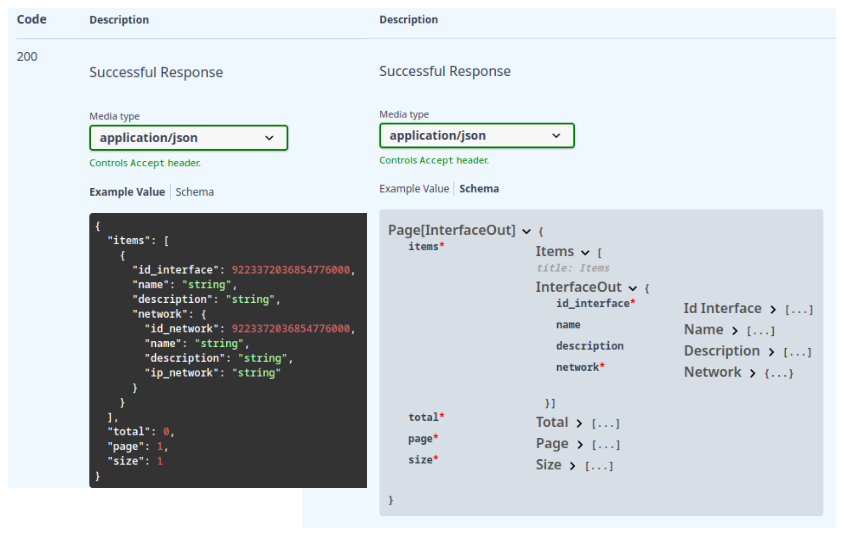
\includegraphics[width=0.78\textwidth]{diag/response_get_interfaces.png}
					\caption{Parámetros GET Interfaces}
					\label{img: response get interfaces}
				\end{center}
			\end{figure}
		\end{itemize}
	
		\pagebreak
		
		\item Ruta \texttt{/networks/\{network\_id\}/interfaces}:
		
		\begin{itemize}
			\item \textbf{Método HTTP}: \texttt{POST}
			\item \textbf{Descripción}: permite crear una interfaz monitorizada, asociada a una red.
			\item \textbf{Parámetros}: \texttt{network\_id}, como identificador de red. Similar a figura \ref{img: parameters post networks}.
		
			\begin{figure}[h!]
				\begin{center}
					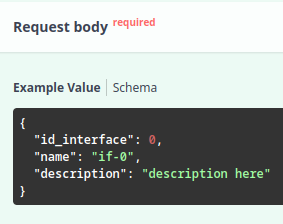
\includegraphics[width=0.4\textwidth]{img/parameters_post_interfaces.png}
					\caption{Parámetros POST Interfaces}
					\label{img: parameters post interfaces}
				\end{center}
			\end{figure}
		
			\begin{figure}[h!]
				\begin{center}
					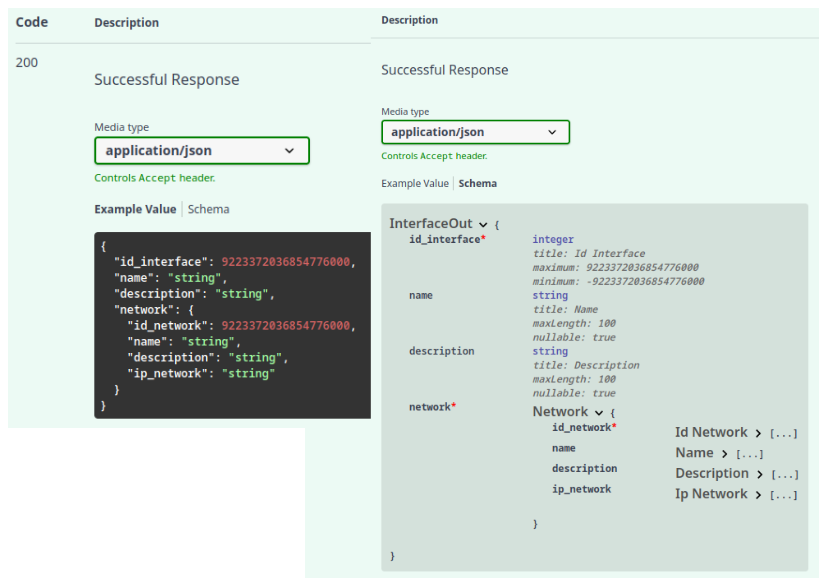
\includegraphics[width=1\textwidth]{diag/response_post_interfaces.png}
					\caption{Parámetros POST Interfaces}
					\label{img: response post interfaces}
				\end{center}
			\end{figure}
		\end{itemize}
	
		\pagebreak
		
		\item Ruta \texttt{/networks/\{network\_id\}/interfaces/\{interface\_id\}}:
		
		\begin{itemize}
			\item \textbf{Método HTTP}: \texttt{GET}
			\item \textbf{Descripción}: devuelve la información de una interfaz, asociada a una red.
			\item \textbf{Parámetros}: \texttt{network\_id} e \texttt{interface\_id}, como identificadores.
			\item \textbf{Respuesta}: similar a la obtenida en la respuesta de \texttt{POST} a \texttt{interfaces}, ver figura \ref{img: response post interfaces}.
		\end{itemize}
	
		\item Ruta \texttt{/networks/\{network\_id\}/interfaces/\{interface\_id\}}:
		
		\begin{itemize}
			\item \textbf{Método HTTP}: \texttt{DELETE}
			\item \textbf{Descripción}: elimina una interfaz de red.
			\item \textbf{Parámetros}: \texttt{network\_id} e \texttt{interface\_id}, como identificadores.
			\item \textbf{Respuesta}: similar a la obtenida en el caso de \texttt{networks}, ver figura \ref{img: response delete network}.
		\end{itemize}
	
		\item Ruta \texttt{/networks/\{network\_id\}/interfaces/\{interface\_id\}}:
		
		\begin{itemize}
			\item \textbf{Método HTTP}: \texttt{PATCH}
			\item \textbf{Descripción}: actualiza una interfaz del sistema, dado un identificador.
			\item \textbf{Parámetros}: \texttt{network\_id} e \texttt{interface\_id}, como identificadores.
			\item \textbf{Respuesta}: equivalente a \ref{img: response post interfaces}, con la información ya modificada.
		\end{itemize}
		
		\begin{figure}[h!]
			\begin{center}
				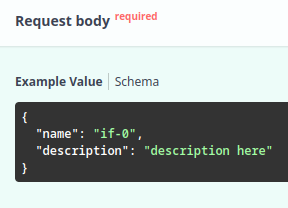
\includegraphics[width=0.45\textwidth]{img/parameters_patch_interfaces.png}
				\caption{Parámetros PATCH Interfaces}
				\label{img: parameters patch interfaces}
			\end{center}
		\end{figure}
	\end{enumerate}
	
	\pagebreak
	
	\subsection{Colección \texttt{Samples}}
	
	\begin{enumerate}
		\item Ruta \texttt{/samples/\{network\_id\}/import\_topology}:
		
		\begin{itemize}
			\item \textbf{Método HTTP}: \texttt{POST}
			\item \textbf{Descripción}: permite subir un archivo tipo \texttt{.csv} que contenga información de más de una interfaz. Las columnas permitidas del \texttt{.csv} son: \texttt{timestamp}, \texttt{interface}, \texttt{TX} y \texttt{RX}. El sistema dará de alta las interfaces asociadas y cargará en la base de datos las muestras para cada una de las interfaces involucradas.
			\item \textbf{Parámetros}: \texttt{network\_id} como identificador de la red a la que se va a subir los datos de monitorización.
			\item \textbf{Respuesta}: una vez se carga la topología, el servidor nos devuelve un mensaje confirmando que se han creado las interfaces de red y que se han subido correctamente los datos a la base de datos.
		\end{itemize}
	
		\item Ruta \texttt{/samples/\{network\_id\}/import\_interface/\{interface\_id\}}:
		
		\begin{itemize}
			\item \textbf{Método HTTP}: \texttt{POST}
			\item \textbf{Descripción}: permite subir un archivo tipo \texttt{.csv} que contenga muestras de tráfico de una única interfaz, especificando si es de tipo \texttt{RX} o \texttt{TX}. Las columnas permitidas del \texttt{.csv} son: \texttt{time} y \texttt{flow}. El sistema subirá la información de las muestras a la base de datos, asociadas a la interfaz de red que especificamos como parámetro.
			\item \textbf{Parámetros}: \texttt{network\_id} e \texttt{interface\_id}, como identificadores tanto de red como de interfaz monitorizada.
			\item \textbf{Respuesta}: una vez cargados los datos de monitorización, el servidor devuelve un mensaje confirmando que se han subido correctamente los datos.
		\end{itemize}
	\end{enumerate}
	
	\subsection{Colección \texttt{Query samples}}
	
	\begin{enumerate}
		\item Ruta \texttt{/query}:
		
		\begin{itemize}
			\item \textbf{Método HTTP}: \texttt{GET}
			\item \textbf{Descripción}: permite consultar la información de monitorización almacenada en el sistema. Además, permite modificar si queremos la salida como \texttt{CSV} o como \texttt{JSON}.
			\item \textbf{Parámetros}: \texttt{network\_id} e \texttt{interface\_id}, como identificadores de los datos a consultar, \texttt{field} para elegir entre interfaz de transmisión (\texttt{TX}) o interfaz de recepción (\texttt{RX}), y \texttt{to\_csv} para elegir entre si queremos la salida en formato \texttt{CSV} (campo en \texttt{true}) o la salida en formato JSON (campo en \texttt{false}).
			\item \textbf{Respuesta}: el servidor devuelve los datos almacenados en el sistema. En función del parámetro \texttt{to\_csv}, la salida será un archivo con formato \texttt{CSV} o un archivo con formato \texttt{JSON}.
		\end{itemize}
	\end{enumerate}
	
	\pagebreak
	
	\subsection{Colección \texttt{Forecast}}
	
	\begin{enumerate}
		\item Ruta \texttt{/forecast}:
		
		\begin{itemize}
			\item \textbf{Método HTTP}: \texttt{POST}
			\item \textbf{Descripción}: permite ejecutar una predicción de tráfico de red sobre una interfaz en específico. Más información en la sección \ref{sec: prophet info}
			\item \textbf{Parámetros}: además del campo \texttt{body} que vemos en la figura \ref{img: parameters post forecast}, tenemos otro parámetro que permite elegir el formato de respuesta del servidor, este parámetro es \texttt{to\_csv} y funciona de manera equivalente que en la ruta de \texttt{/query}.
			\item \textbf{Respuesta}: el servidor devuelve la serie temporal completa, tanto la almacenada como los datos predichos. En función del parámetro \texttt{to\_csv}, la salida tendrá formato \texttt{CSV} (ver figura \ref{img: output forecast csv}) o bien \texttt{JSON} (ver figura \ref{img: output forecast json}).
			
			\begin{figure}[h!]
				\begin{center}
					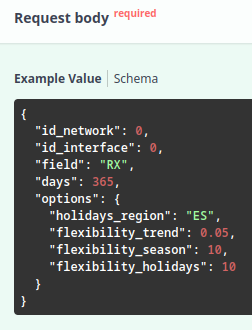
\includegraphics[width=0.25\textwidth]{img/parameters_post_forecast.png}
					\caption{Parámetros POST Forecast}
					\label{img: parameters post forecast}
				\end{center}
			\end{figure}
		
			\begin{figure}[h!]
				\begin{center}
					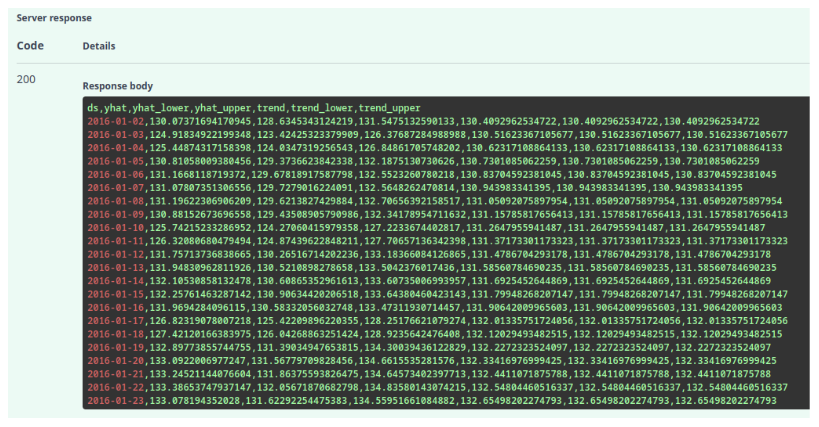
\includegraphics[width=0.91\textwidth]{img/output_forecast_csv.png}
					\caption{Respuesta del servidor de una predicción de tráfico, en formato \texttt{CSV}.}
					\label{img: output forecast csv}
				\end{center}
			\end{figure}
		
			\pagebreak
			
			\begin{figure}[h!]
				\begin{center}
					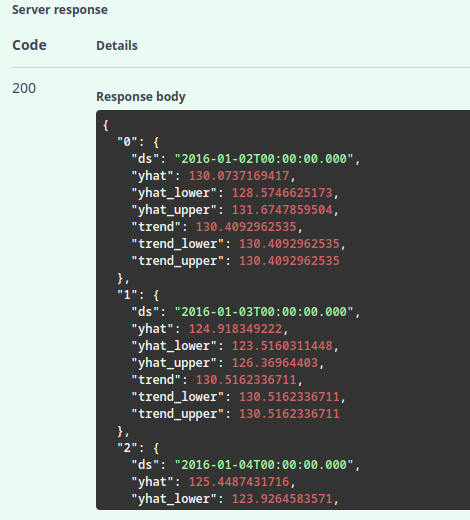
\includegraphics[width=0.6\textwidth]{img/output_forecast_json.png}
					\caption{Respuesta del servidor de una predicción de tráfico, en formato \texttt{JSON}.}
					\label{img: output forecast json}
				\end{center}
			\end{figure}
		\end{itemize}
	\end{enumerate}
	
	\pagebreak
	
	\chapter{Validación del sistema}
	
	\noindent En este capítulo vamos a demostrar y validar el funcionamiento del sistema, además de verificar que este cumple con los objetivos propuestos para el trabajo. A modo de resumen, las pruebas realizadas son las siguientes:
	
	\begin{enumerate}
		\item Crear una red a monitorizar.
		\item Crear una interfaz dentro de una red a monitorizar.
		\item Cargar muestras en interfaz de red.
		\item Cargar una topología de red sobre una red a monitorizar.
		\item Consultar datos de monitorización almacenados en el sistema.
		\item Ejecutar una predicción de tráfico de un año.
		%\item Ejecutar una predicción de tráfico de 2 años.
	\end{enumerate}

	\section{Crear una red a monitorizar}
	
	\begin{figure}[h!]
		\begin{center}
			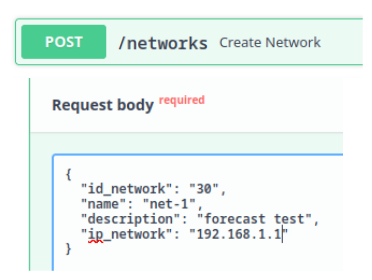
\includegraphics[width=0.5\textwidth]{diag/request_create_net.png}
			\caption{Petición para crear red a monitorizar.}
			\label{img: request create net}
		\end{center}
	\end{figure}
	
	\pagebreak
	
	\noindent Tal y como vemos en la figura \ref{img: request create net}, realizamos una petición \texttt{POST} a la ruta \texttt{/networks}, con el \texttt{request body} que vemos también en la figura. De este modo, en el sistema se creará una red a monitorizar llamada \texttt{net-1} con el identificador \texttt{30}. \\
	
	\noindent La respuesta recibida por el servidor ante esta petición la podemos ver en la figura \ref{img: response create net (validate)}.
	
	\begin{figure}[h!]
		\begin{center}
			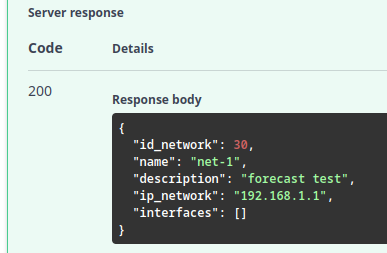
\includegraphics[width=0.5\textwidth]{img/response_create_net.png}
			\caption{Respuesta servidor después de crear red.}
			\label{img: response create net (validate)}
		\end{center}
	\end{figure}

	\section{Crear una interfaz de red monitorizada}
	
	\begin{figure}[h!]
		\begin{center}
			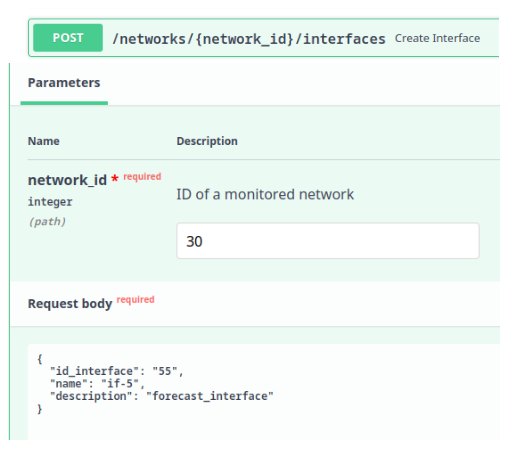
\includegraphics[width=0.65\textwidth]{diag/request_create_if.png}
			\caption{Petición para crear una interfaz de red monitorizada.}
			\label{img: request create if (validate)}
		\end{center}
	\end{figure}

	\pagebreak
	
	\noindent A la red que acabamos de crear (\texttt{net-1}, con id \texttt{30}), le añadimos una interfaz de red monitorizada con el identificador \texttt{55}. Dicha interfaz de red monitorizada tiene por nombre \texttt{if-5}. Ver figura \ref{img: request create if (validate)}. \\
	
	\noindent La respuesta recibida por el servidor ante esta petición la podemos ver en la figura \ref{img: response create if (validate)}.
	
	\begin{figure}[h!]
		\begin{center}
			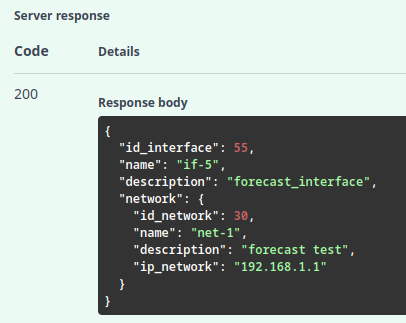
\includegraphics[width=0.65\textwidth]{img/response_create_if.png}
			\caption{Respuesta del servidor después de crear una interfaz de red.}
			\label{img: response create if (validate)}
		\end{center}
	\end{figure}
	
	\section{Cargar muestras en interfaz de red}
	\label{sec: load data if}
	
	\noindent El siguiente paso para validar el sistema es cargar datos de monitorización. Para ello se propuso la opción de generar un \texttt{dataset} de datos sintéticos en el que se puedan aplicar ciertos efectos de tendencia o estacionales, de modo que se pueda validar la correcta predicción del tráfico. Los pasos que se han seguido para generar dicho \texttt{dataset} se pueden ver en anexo I (\ref{sec: anexo 1 dataset}). \\
	
	\noindent En este caso, utilizamos un \texttt{dataset} de dos años con muestras de tráfico cada 5 minutos. En la figura \ref{img: synthetic dataset two year} podemos ver que forma tiene los datos de monitorización. Este \texttt{dataset} lo subimos al sistema para que se añadan a la interfaz monitorizada con identificación \texttt{55}. \\
	
	\noindent En la figura \ref{img: request import if (validate)} podemos ver como se selecciona el archivo de muestras sintéticas, y además se realiza la petición para que las muestras se cargue con muestras de monitorización de recepción (ver detalle en el campo \texttt{field}). \\
	
	\noindent Una vez enviamos la petición, el servidor tarda aproximadamente 5-6 segundos en dar una respuesta. Para este caso, el \texttt{dataset} de dos años tiene un peso de 5.8 MB. En la figura \ref{img: response import if (validate)} podemos ver la respuesta recibida por el servidor. \\
	
	\pagebreak

	\begin{figure}[h!]
		\begin{center}
			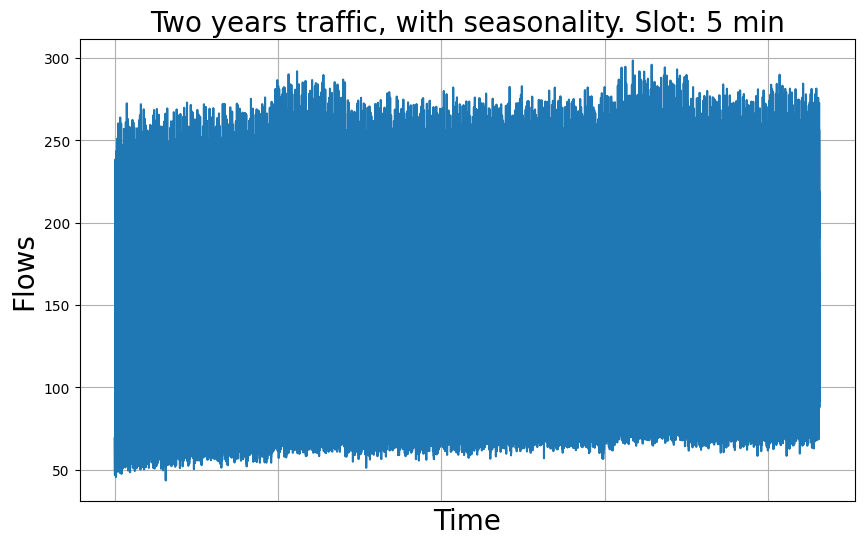
\includegraphics[width=0.75\textwidth]{img/dataset_synt_1.png}
			\caption{Representación datos sintéticos de dos años.}
			\label{img: synthetic dataset two year}
		\end{center}
	\end{figure}
	
	\begin{figure}[h!]
		\begin{center}
			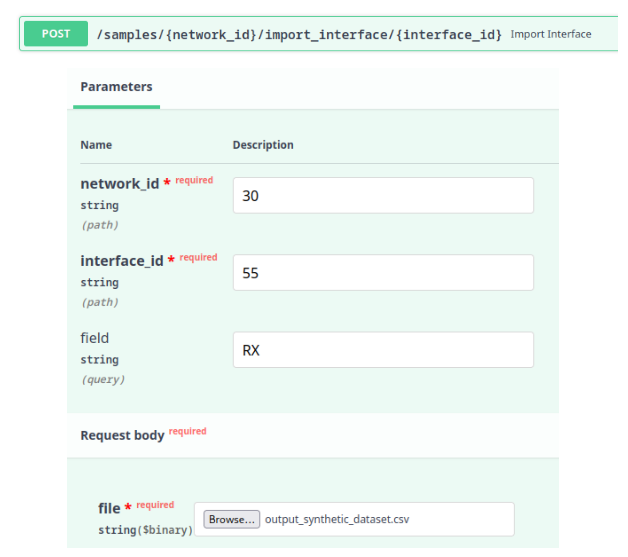
\includegraphics[width=0.8\textwidth]{diag/request_import_if.png}
			\caption{Petición para añadir muestras de monitorización a una interfaz.}
			\label{img: request import if (validate)}
		\end{center}
	\end{figure}
	
	\pagebreak
	
	\begin{figure}[h!]
		\begin{center}
			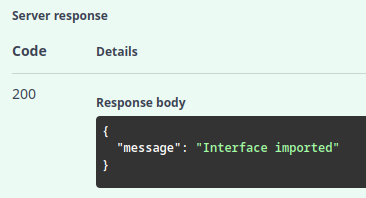
\includegraphics[width=0.5\textwidth]{img/response_import_if.png}
			\caption{Respuesta del servidor una vez ha completado la petición de importar datos de monitorización.}
			\label{img: response import if (validate)}
		\end{center}
	\end{figure}

	\noindent Llegados a este punto, es interesante comprobar si de verdad se han subido los datos de monitorización al sistema. Recapitulando de los modelos de datos, los datos de monitorización están almacenados en la base de datos InfluxDB, por lo que podemos hacer uso del portal web que viene por defecto en la aplicación para comprobar si se han subido los datos correctamente. Una vez accedemos al portal web, y seleccionamos el \texttt{bucket} de nuestra aplicación, procedemos a buscar los datos de monitorización que acabamos de subir. En la figura \ref{img: influxdb data 1} podemos ver una captura de pantalla de la aplicación web de InfluxDB y los datos de monitorización que acabamos de subir.
	
	\begin{figure}[h!]
		\begin{center}
			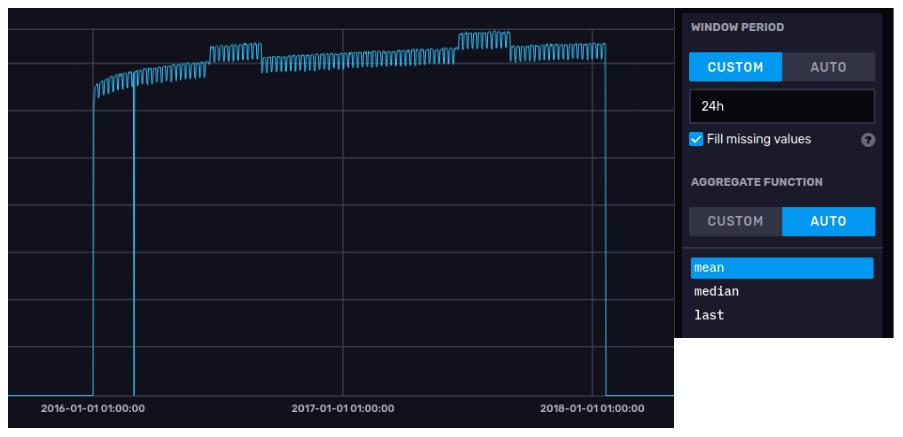
\includegraphics[width=1\textwidth]{diag/influxdb_data_1.png}
			\caption{Captura InfluxDB. Datos de monitorización correctamente subidos al sistema.}
			\label{img: influxdb data 1}
		\end{center}
	\end{figure}
	
	\pagebreak
	
	\section{Cargar una topología de red}
	
	\noindent Por otro lado, otra forma de cargar muestras de monitorización a una red es utilizando la ruta: \\
	 \texttt{/samples/\{network\_id\}/import\_topology}, ya que permite subir información de más de una interfaz de forma simultanea. Para ello, tenemos que subir un archivo \texttt{CSV} que tenga las siguientes columnas:
	 
	 \begin{itemize}
	 	\item \texttt{timestamp}. Valor temporal de la muestra, cada 5 minutos.
	 	\item \texttt{interface}. Nombre de la interfaz monitorizada.
	 	\item \texttt{TX}. Valor de tráfico de red en la interfaz de transmisión.
	 	\item \texttt{RX}. Valor de tráfico de red en la interfaz de recepción.
	 \end{itemize}
 
 	\noindent Para este ejemplo, hemos generado un pequeño archivo de monitorización que vamos a subir a una red de monitorización que previamente tenemos creada (en este caso, red con identificación \texttt{100}). Una vez el sistema lea el archivo, creará las interfaces que sean necesarias para dar lugar a la topología. Una vez termine, subirá los datos de monitorización para cada una de las interfaces. \\
 	
 	\begin{figure}[h!]
 		\begin{center}
 			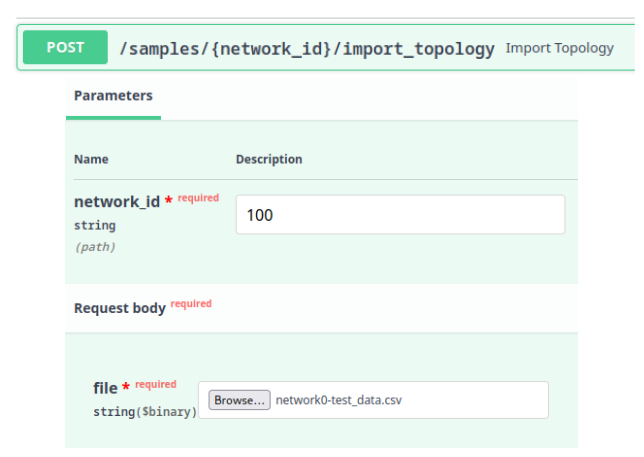
\includegraphics[width=0.55\textwidth]{diag/request_topology_1.png}
 			\caption{Petición para cargar una topología en la red \texttt{100}.}
 			\label{img: request topology 1}
 		\end{center}
 	\end{figure}
 
 	\begin{figure}[h!]
 		\begin{center}
 			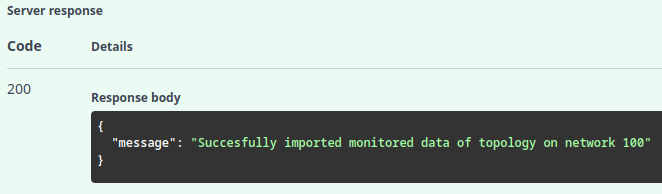
\includegraphics[width=0.75\textwidth]{img/response_topology_1.png}
 			\caption{Respuesta del servidor al cargar una topología de red.}
 			\label{img: response topology 1}
 		\end{center}
 	\end{figure}
	
	\pagebreak
	
	\noindent Para comprobar que se ha subido correctamente los datos, accedemos al portal web de InfluxDB. En la figura \ref{img: influxdb topology 1} podemos ver como los datos se han subido correctamente. En esta captura también podemos comprobar como se agrupan los datos dentro de la base de datos de tipo serie temporal. 
	
	\begin{figure}[h!]
		\begin{center}
			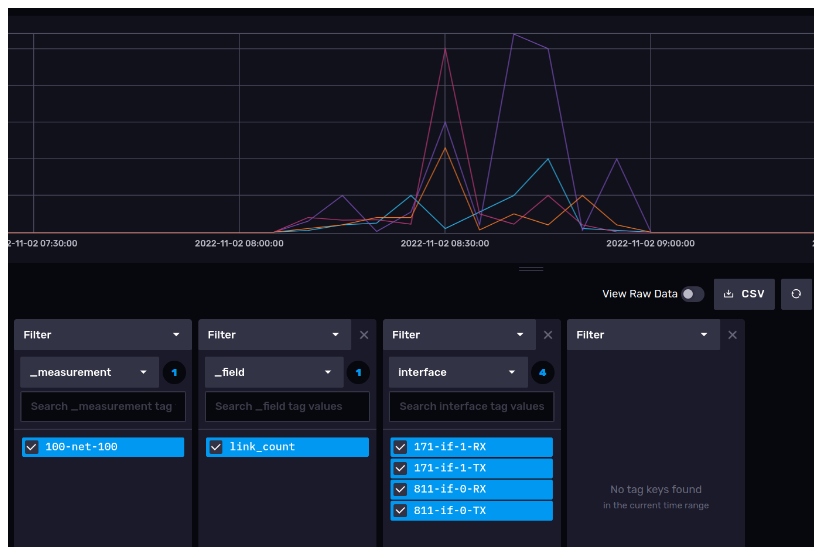
\includegraphics[width=1\textwidth]{diag/influxdb_topology_1.png}
			\caption{Respuesta del servidor al cargar una topología de red.}
			\label{img: influxdb topology 1}
		\end{center}
	\end{figure}
	
	\section{Consultar datos de monitorización}
	
	\noindent Otra funcionalidad importante del sistema es que además de poder cargar información de tráfico, podemos recuperar dicha información de modo que el servidor nos devuelva la información de monitorización asociada a la petición que nosotros le hemos realizado. Para ello, utilizamos la ruta \texttt{/query} con el método \texttt{GET}. \\
	
	\noindent En este caso, vamos a validar que el sistema correctamente nos puede dar la información de monitorización de una red con identificador \texttt{100}, que tiene una interfaz con identificador \texttt{171}, y elegimos que nos devuelva los datos de recepción (\texttt{field} equivalente a \texttt{RX}). Ver figura \ref{img: parameters query 1}. \\
	
	\noindent La respuesta del servidor puede ser en formato \texttt{JSON} o \texttt{CSV} en función del parámetro \texttt{to\_csv} de la petición. En la figura \ref{img: response query 1} podemos ver como el servidor nos devuelve los datos de la interfaz solicitada en formato \texttt{JSON}.
	
	\pagebreak
	
	\begin{figure}[h!]
		\begin{center}
			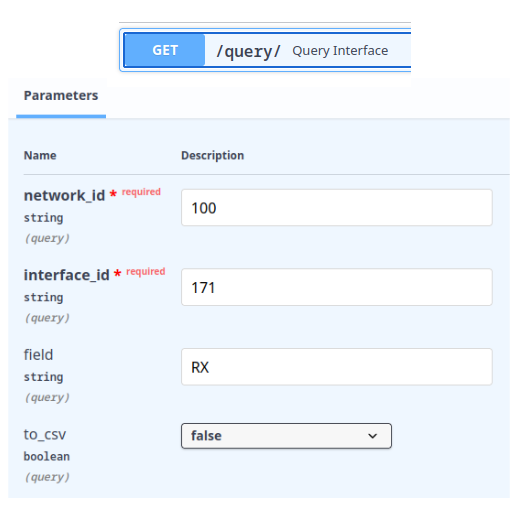
\includegraphics[width=0.6\textwidth]{diag/parameters_query_1.png}
			\caption{Petición para consultar datos de monitorización del sistema.}
			\label{img: parameters query 1}
		\end{center}
	\end{figure}

	\begin{figure}[h!]
		\begin{center}
			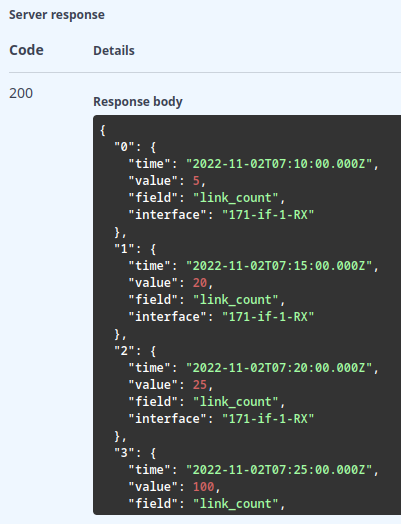
\includegraphics[width=0.45\textwidth]{img/response_query_1.png}
			\caption{Respuesta del servidor al consultar datos de monitorización, salida en formato \texttt{JSON}.}
			\label{img: response query 1}
		\end{center}
	\end{figure}
	
	\pagebreak
	
	\section{Predicción de tráfico de un año}
	
	\noindent En este punto, queremos realizar una predicción de tráfico de red a partir de las muestras subidas al sistema en el apartado \ref{sec: load data if}. Las muestras subidas van desde 2016 hasta inicios de 2018, por lo que queremos predecir desde inicios de 2018 hasta inicios de 2019. \\
	
	\noindent En la figura \ref{img: request forecast validate} podemos ver como se realiza la petición para la predicción de tráfico. 
	
	\begin{figure}[h!]
		\begin{center}
			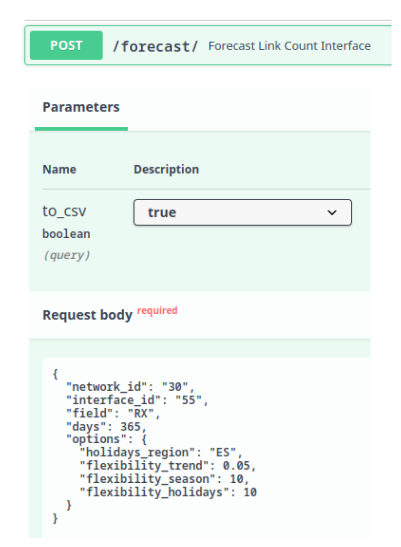
\includegraphics[width=0.4\textwidth]{diag/request_forecast_validate1.png}
			\caption{Petición para ejecutar una predicción de tráfico.}
			\label{img: request forecast validate}
		\end{center}
	\end{figure}

	\begin{figure}[h!]
		\begin{center}
			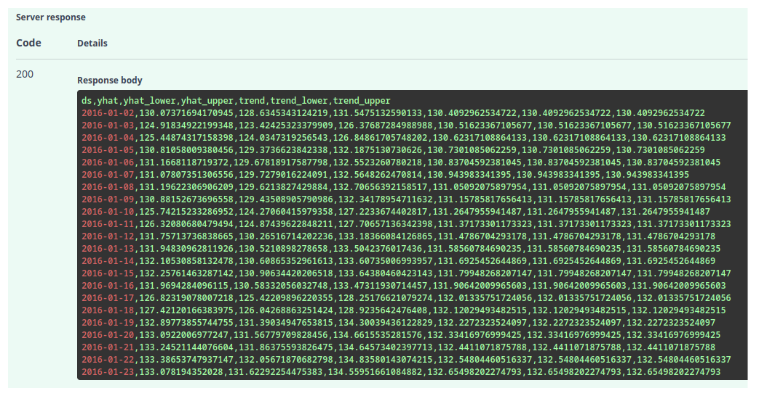
\includegraphics[width=0.85\textwidth]{diag/output_forecast_validate_csv.png}
			\caption{Respuesta del servidor de ejecución predicción (salida en \texttt{CSV}).}
			\label{img: output forecast validate csv}
		\end{center}
	\end{figure}
	
	\pagebreak
	
	\noindent Tal y como podemos ver en la figura \ref{img: output forecast validate csv}, si activamos la opción de \texttt{to\_csv}, la respuesta del servidor estará preparada para ser leída como un \texttt{CSV}, si no lo activamos la salida será en formato \texttt{JSON} (ver figura \ref{img: output forecast validate json}). Los campos de salida son:
	
	\begin{itemize}
		\item \texttt{ds}. Valor temporal de la muestra.
		\item \texttt{yhat}. Valor medio en ese instante temporal.
		\item \texttt{yhat\_lower}. Valor mínimo en ese instante temporal.
		\item \texttt{yhat\_upper}. Valor máximo en ese instante temporal.
		\item \texttt{trend}. Valor medio de la tendencia.
		\item \texttt{trend\_lower}. Valor mínimo de la tendencia.
		\item \texttt{trend\_upper}. Valor máximo de la tendencia.
	\end{itemize}

	\begin{figure}[h!]
		\begin{center}
			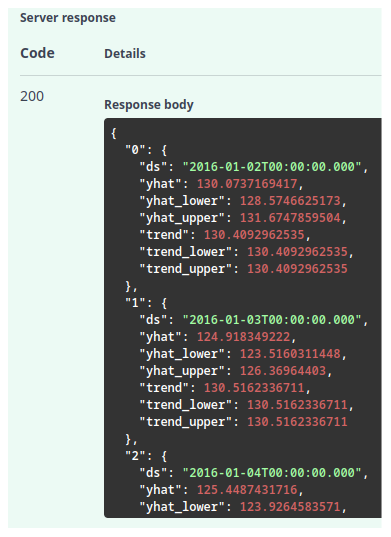
\includegraphics[width=0.6\textwidth]{diag/output_forecast_validate_json.png}
			\caption{Respuesta del servidor de ejecución predicción (salida en \texttt{JSON}).}
			\label{img: output forecast validate json}
		\end{center}
	\end{figure}
	
	\pagebreak
	
	\noindent Para comprobar la predicción realizada, procedemos a representar los datos que hemos recibido en la respuesta del servidor. Para ello, vemos las figuras \ref{img: graph forecast 1} y \ref{img: graph forecast 2}, en las que podemos comprobar que el \texttt{dataset} ahora dura hasta principios de 2019, y que además ha podido predecir correctamente la tendencia de crecimiento exponencial anual y los efectos de tráfico añadidos sintéticamente (como por ejemplo, efecto fin de semana o el efecto verano). \\
	
	\begin{figure}[h!]
		\begin{center}
			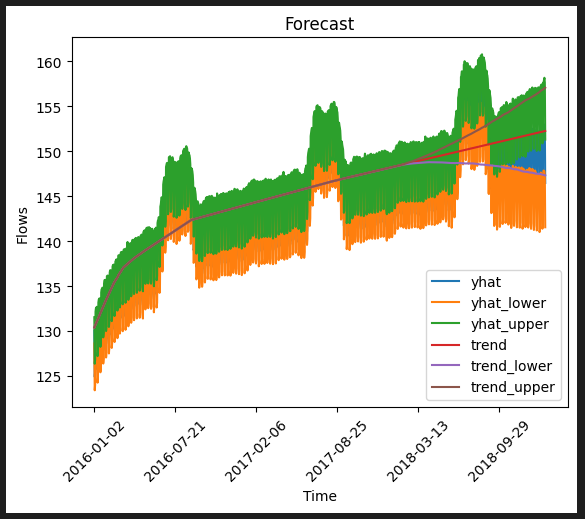
\includegraphics[width=0.55\textwidth]{img/graph_forecast_1.png}
			\caption{Gráfica datos de salida de la predicción de tráfico.}
			\label{img: graph forecast 1}
		\end{center}
	\end{figure}

	\begin{figure}[h!]
		\begin{center}
			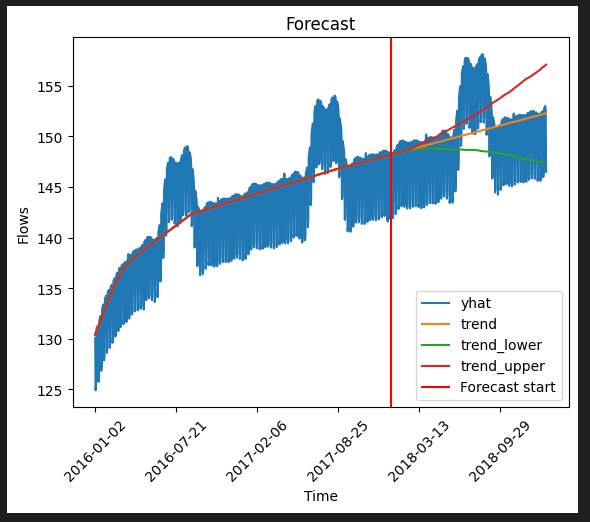
\includegraphics[width=0.55\textwidth]{img/graph_forecast_2.png}
			\caption{Gráfica datos de salida de la predicción de tráfico. A la izquierda de la linea roja, datos de muestras; a la derecha, datos predichos por el sistema.}
			\label{img: graph forecast 2}
		\end{center}
	\end{figure}
	
	\pagebreak
	
	\chapter{Conclusiones y propuestas futuras}
	
	\noindent En este capítulo vamos a comentar las conclusiones obtenidas durante la realización del presente trabajo. \\
	
	\noindent En primer lugar, se ha profundizado en el concepto de microservicios y APIs, permitiendo desplegar una aplicación que está alineada completamente con estos conceptos. Además, se ha demostrado que el despliegue tanto en un entorno de desarrollo, como en un entorno de producción, es relativamente sencillo ya que hacemos uso de las herramientas \texttt{Docker} y \texttt{docker-compose}. \\
	
	\noindent Por otro lado, gracias al framework FastAPI, la aplicación tiene implementadas herramientas de documentación del estándar de OpenAPI. Esto es importante ya que permite que otras aplicaciones puedan hacer uso de la API como servicio, de modo que aplicaciones más grandes puedan aumentar su funcionalidad de manera sencilla, simplemente conectándose con el servicio propuesto en este trabajo. Además, esta documentación también ha sido clave para la validación del desarrollo, ya que permite ejecutar peticiones y comprobar la funcionalidad de la aplicación. \\

	\noindent En el tema de bases de datos, se ha podido comprobar la importancia de elegir las bases de datos en función del tipo de dato que queremos almacenar en nuestra aplicación. Es por esto por lo que datos relacionados entre sí, es ideal usar una base de datos tipo SQL. Para las muestras de monitorización, que son mucho más volumen de información, y están referidas a un instante temporal; es importante disponer de una base de datos que pueda manejar esta información. Es por ello, por lo que elegimos InfluxDB para almacenar series temporales, y como hemos podido comprobar que su desempeño es brillante y muy adecuado para la tarea encomendada. \\
	
	\noindent En relación a la predicción de tráfico de red, se realizó la investigación acerca de las opciones para predecir series temporales, y si bien es cierto que de primeras \texttt{Prophet} era prometedor, una vez terminada la aplicación, se puede comprobar el potencial de esta herramienta, ya que permite tener las predicciones en poco tiempo, con un \texttt{dataset} de entrenamiento bajo, y además, permite configurar de manera dinámica los días a predecir. Esta característica es muy importante, ya que nos permite realizar predicciones a diferentes escalas temporales, y dependiendo de la escala, podemos dar una utilidad a los datos ofrecidos por la aplicación. \\
	
	\noindent En resumen, podemos concluir que el presente trabajo ha cumplido con los objetivos propuestos, ya que satisfactoriamente se ha desarrollado una aplicación capaz de almacenar datos de red y generar una predicción en función de dichos datos, además de cumplir los requisitos de software establecidos para facilitar la integración de la herramienta con otros servicios. \\
	
	%\pagebreak
	
	\noindent \textbf{\large Propuestas futuras} \\
	
	\noindent Algunas de las líneas de investigación que pueden resultar interesantes para continuar con este proyecto, son las siguientes:
	
	\begin{itemize}
		\item Extender la funcionalidad de la aplicación para permitir la importación de datos de monitorización de herramientas de planificación de red. De este modo, se le daría un valor añadido a la funcionalidad de predicción, ya que se podría explotar la información generada por herramientas más profesionales.
		
		\item Añadir la funcionalidad de que los \texttt{endpoints} que requieren más tiempo de ejecución (como por ejemplo, el de predicción) utilicen la metodología de \texttt{SSE} (\textbf{S}erver \textbf{S}ide \textbf{E}vent), esto permite a la aplicación informar al cliente del progreso para completar la petición realizada al servidor. Esto es muy interesante ya que permitiría una mejor implementación en aplicaciones que consuman el servicio propuesto, ya que pueden estimar el tiempo de procesado, y mostrar a un usuario en que estado se encuentra la petición.
		
		\item Incluir nuevos parámetros en las peticiones de predicción o consultas al sistema, permitiendo ser más selectivos con la información, además de poder integrar nuevas funcionalidades como modificar el percentil a aplicar, buscar la hora cargada, etc. 
		
		\item Profundizar en despliegues basados en tecnología ``cloud'' con Kubernetes, facilitando el despliegue de los microservicios, además de permitir el autoescalado de los recursos. De modo que si una instancia de nuestra aplicación en un momento determinado requiere más recursos, puede tenerlos de manera automática, agilizando de esta manera la ejecución de la predicción.
	\end{itemize}
	
	\pagebreak
	
	\chapter{Bibliografía}
	
	\subsection*{Enlaces y referencias}
	\addcontentsline{toc}{section}{Enlaces y referencias}
	
	\begin{enumerate}
		% 1
		\item 
		\label{bib: apuntes OeIR}
		\href{https://teleco.upct.es/guia-docente/211101007}{Apuntes de la asignatura \texttt{Operación e Ingenieria de Red}, del Master Universitario en Ingenieria de Telecomunicaciones de la UPCT}
		
		% 2
		\item
		\label{bib: what is api}
		\href{https://aws.amazon.com/es/what-is/api/}{¿Qué es una API?}
		
		% 3
		\item
		\label{bib: microservices}
		\href{https://learn.microsoft.com/en-us/azure/architecture/guide/architecture-styles/microservices}{Microservice architecture style}
		
		% 4
		\item
		\label{bib: relational database}
		\href{https://cloud.google.com/learn/what-is-a-relational-database}{What is a relational database?}
				
		% 5
		\item
		\label{bib: postgresql}
		\href{https://www.postgresql.org/}{PostgreSQL}
		
		% 6
		\item
		\label{bib: influxdb doc}
		\href{https://www.stackhero.io/en/services/InfluxDB/documentations/Introduction#differences-between-influxdb-and-relational-sql-databases}{InfluxDB: Introduction}
		
		% 7
		\item
		\label{bib: influxdb doc vs sql}
		\href{https://archive.docs.influxdata.com/influxdb/v1.2/concepts/crosswalk/}{InfluxDB: Comparison to SQL}
		
		% 8
		\item
		\label{bib: python doc}
		\href{https://www.python.org/}{Python}
		
		% 9
		\item
		\label{bib: fastapi doc}
		\href{https://fastapi.tiangolo.com/}{FastAPI framework}
		
		% 10
		\item
		\label{bib: openapi}
		\href{https://github.com/OAI/OpenAPI-Specification}{GitHub: OpenAPI-Specification}
		
		% 11
		\item
		\label{bib: json schema}
		\href{https://json-schema.org/}{JSON Schema}
		
		% 12
		\item
		\label{bib: prophet doc}
		\href{https://facebook.github.io/prophet/}{Prophet}
		
		% 13
		\item
		\label{bib: docker compose doc}
		\href{https://docs.docker.com/compose/}{Docker Compose Overview}
		
		% 14
		\item
		\label{bib: traefik webpage}
		\href{https://traefik.io/traefik/}{Traefik Webpage}
		
		% 15
		\item
		\label{bib: traefik wiki}
		\href{https://doc.traefik.io/traefik/}{Traefik Wiki}
		
		% 16
		\item
		\label{bib: factory method}
		\href{https://www.geeksforgeeks.org/factory-method-python-design-patterns/}{Factory Method - Python Design Patterns}
		
		% 17
		\item
		\label{bib: fastapi doc bigger apps}
		\href{https://fastapi.tiangolo.com/tutorial/bigger-applications/}{FastAPI Doc: Bigger Applications}
		
		% 18
		\item
		\label{bib: orm python}
		\href{https://www.fullstackpython.com/object-relational-mappers-orms.html}{Object-relational Mappers (ORMs)}
		
		% 19
		\item
		\label{bib: fastapi orm}
		\href{https://fastapi.tiangolo.com/tutorial/sql-databases/#orms}{FastAPI Doc: SQL (Relational) Databases. ORM}
		
		% 20
		\item
		\label{bib: fastapi migrations}
		\href{https://fastapi.tiangolo.com/tutorial/sql-databases/#migrations}{FastAPI Doc: SQL (Relational) Databases. Migrations}
		
		% 21
		\item
		\label{bib: prophet parameters}
		\href{https://facebook.github.io/prophet/docs/diagnostics.html#hyperparameter-tuning}{Prophet Doc: Hyperparameter-tuning}
		
		% 22
		\item
		\label{bib: prophet trend flex}
		\href{https://facebook.github.io/prophet/docs/trend_changepoints.html#adjusting-trend-flexibility}{Prophet Doc: Adjusting trend flexibility}
		
		% 22
		\item
		\label{bib: cisco white paper}
		\href{https://www.cisco.com/c/en/us/solutions/collateral/executive-perspectives/annual-internet-report/white-paper-c11-741490.html}{Cisco Annual Internet Report (2018-2023) White paper}
		
		
	\end{enumerate}

	\vspace{20px}
	
	\subsection*{Figuras}
	\addcontentsline{toc}{section}{Imagenes}

	\begin{enumerate}
		
		% 1
		\item
		\label{bib_img: microservice architecture}
		\href{https://xbsoftware.com/blog/microservices-vs-monolithic-architecture/}{Monolithic vs Microservices Architecture}
		
		% 2
		\item
		\label{bib_img: example sql}
		\href{https://xbsoftware.com/blog/main-types-of-database-management-systems/}{Relational Databases}
		
		% 3
		\item
		\label{bib_img: influxdb logo}
		\href{https://www.influxdata.com/}{InfluxDB}
		
		% 4
		\item
		\label{bib_img: python logo}
		\href{https://www.python.org/}{Python}
		
		% 5
		\item
		\label{bib_img: fastapi logo}
		\href{https://fastapi.tiangolo.com/}{FastAPI}
		
		% 6
		\item
		\label{bib_img: prophet logo}
		\href{https://facebook.github.io/prophet/}{Prophet}
		
		% 7
		\item
		\label{bib_img: docker architecture}
		\href{https://docs.docker.com/get-started/overview/}{Docker Docs: Get Started}
		
		% 8
		\item
		\label{bib_img: traefik capture}
		\href{https://traefik.io/traefik/}{Traefik website}
		
	\end{enumerate}
	
	\pagebreak
	
	\chapter*{Anexos}
	\addcontentsline{toc}{chapter}{Anexos}
	
	\section*{Anexo I. Generación \texttt{dataset} sintético}
	\addcontentsline{toc}{section}{Anexo I. Generación dataset sintético}
	\label{sec: anexo 1 dataset}
	
	\noindent Con el objetivo de tener un \texttt{dataset} que se adapte lo suficiente a la situación a validar por nuestra aplicación, se decide generar un \texttt{dataset} sintético, en el que podamos modificar ciertos parámetros que provoquen cambios en el mismo (por ejemplo, cambio de ruido, cambio en las tendencias...). \\
	
	\noindent Para dar lugar a un \texttt{dataset} sintético, se utiliza el lenguaje de programación Python, y se siguen los siguientes pasos: 
	
	\begin{enumerate}
		\item Generamos un archivo tipo \texttt{.csv} de dos columnas (\texttt{time} y \texttt{flow}) que simulan el tráfico de red en una interfaz durante un día. \\
		
		\noindent En este caso, tenemos dos opciones, la primera sería generar un dato de tráfico cada hora (ver figura \ref{img: anexo 1}), y la segunda generar un dato de tráfico cada 5 minutos (ver figura \ref{img: anexo 2}). Este último sería la opción más cercana a la realidad, ya que los datos de tráfico que aporta SNMP se obtienen cada 5 minutos por convenio.
		
		\begin{figure}[h!]
			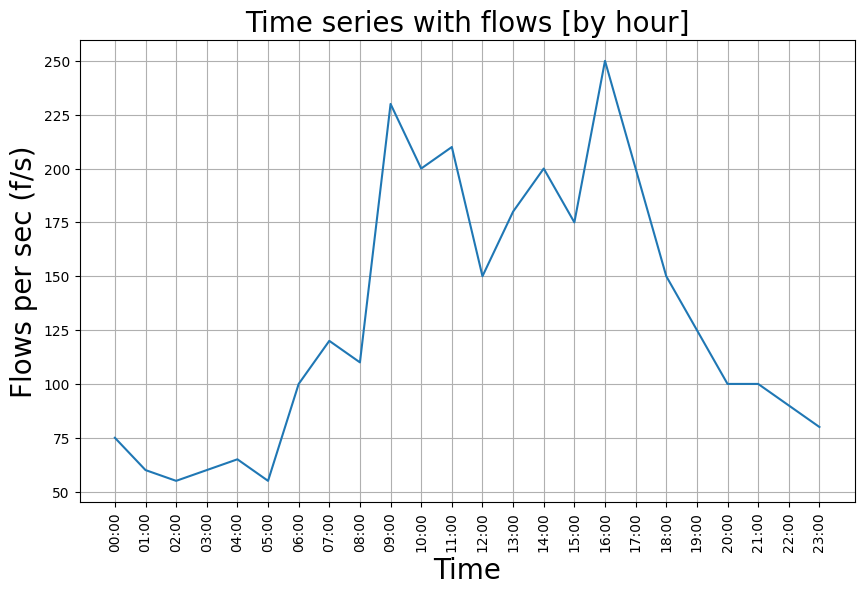
\includegraphics[width=0.8\textwidth, center]{img/anexo_1.png}
			\caption{Simulación de tráfico de red. Un día, dividido por horas.}
			\label{img: anexo 1}
		\end{figure}
	
		\pagebreak
		
		\begin{figure}[h!]
			\includegraphics[width=0.85\textwidth, center]{img/anexo_2.png}
			\caption{Simulación de tráfico de red. Un día, dividido por \texttt{slots} de 5 minutos.}
			\label{img: anexo 2}
		\end{figure}
	
		\item A partir de estos datos, generamos una semana. En esta etapa, añadimos la primera regla: los fines de semana el tráfico se ve reducido, en comparación con el resto de la semana. Ver figura \ref{img: anexo 3}.
		
		\begin{figure}[h!]
			\includegraphics[width=0.85\textwidth, center]{img/anexo_3.png}
			\caption{Simulación de tráfico de red. Una semana con \texttt{slots} de 5 minutos. Reducción de tráfico en el fin de semana}
			\label{img: anexo 3}
		\end{figure}
	
		\pagebreak
		
		\item A los datos anteriores, podemos añadir las reglas de: 
		\begin{itemize}
			\item \textbf{Ruido}. Sumamos ruido blanco a la muestra sintética, de este modo podemos aumentar la varianza de los datos.
			
			\item \textbf{Tendencia}. Aplicamos un crecimiento exponencial a la serie temporal. En el caso de tráfico en red, buscamos seguir el dato de CAGR (Tasa de crecimiento anual compuesto), propuesto por Cisco [\ref{bib: cisco white paper}], por lo que lo implementamos con una exponencial de crecimiento 27\%.
			
		\end{itemize}
	
		\noindent El resultado al aplicar estas reglas se puede ver en la figura \ref{img: anexo 4}.
		
		\begin{figure}[h!]
			\includegraphics[width=0.9\textwidth, center]{img/anexo_4.png}
			\caption{Simulación de tráfico de red. Una semana con \texttt{slots} de 5 minutos. Reducción de tráfico en fin de semana, tendencia exponencial y ruido blanco.}
			\label{img: anexo 4}
		\end{figure}
	
		\item Llegados a este punto, podemos extender el paso anterior para tener muestras durante un mes completo. Esto daría lugar a la figura \ref{img: anexo 5}.
		
		\item Por último, podemos extender el punto anterior si generamos un año completo. Además, en este punto podemos añadir otra regla más: el tráfico en verano aumenta. De esta manera, podemos observar un efecto de incremento en los meses de Junio, Julio y Agosto. El resultado de esta regla lo podemos ver en la figura \ref{img: anexo 6}. \\
		
		\noindent Además, si aplicamos el percentil 95 a la serie temporal de un año, podemos ver más claramente las diferentes reglas aplicadas (ver figura \ref{img: anexo 7}).
		
		\pagebreak
		
		\begin{figure}[h!]
			\includegraphics[width=0.9\textwidth, center]{img/anexo_5.png}
			\caption{Simulación de tráfico de red. Un mes de datos, manteniendo reglas aplicadas.}
			\label{img: anexo 5}
		\end{figure}
	
		\begin{figure}[h!]
			\includegraphics[width=0.9\textwidth, center]{img/anexo_6.png}
			\caption{Simulación de tráfico de red. Un año de datos, se añade la regla del incremento de tráfico en verano.}
			\label{img: anexo 6}
		\end{figure}
	
		\pagebreak
	
		\begin{figure}[h!]
			\includegraphics[width=0.9\textwidth, center]{img/anexo_7.png}
			\caption{Simulación de tráfico de red. Un año de datos, se aplica el percentil 95 para cada día.}
			\label{img: anexo 7}
		\end{figure}
	
		\noindent Una vez llegados a este punto, tenemos un \texttt{dataset} sintético de un año (en formato \texttt{.csv}), en el que podemos modificar diferentes parámetros. De esta manera, podemos validar la predicción de tráfico de nuestra aplicación. \\
	\end{enumerate}
	
\end{document}